%%% Single-sided print version:
\documentclass[11pt,a4paper]{report}
\usepackage[top=25mm,bottom=25mm,right=25mm,left=30mm,head=12.5mm,foot=12.5mm]{geometry}
\let\openright=\clearpage

%%% Double-sided print version (uncomment if needed):
%\documentclass[11pt,a4paper,twoside,openright]{report}
%\usepackage[top=25mm,bottom=25mm,right=25mm,left=30mm,head=12.5mm,foot=12.5mm]{geometry}
%\let\openright=\cleardoublepage

%%% VARIABLE DEFINITIONS
\def\TypPrace{BP}                % bachelor thesis
\def\Jazyk{eng}                  % english

%%% Package definitions and macros (see inside file)
%%% This file contains definitions of various useful macros and environments %%%
%%% Assign additional macros here so that they do not interfere with other files. %%%

\usepackage{ifpdf}
\usepackage{ifxetex}
\usepackage{ifluatex}
\usepackage{ifthen}

%% Fonts and language setup
\ifthenelse{\boolean{xetex}\OR\boolean{luatex}}
   { % use fontspec and OpenType fonts with utf8 engines
			\usepackage[czech,slovak,english]{babel}
			\usepackage[autostyle,english=british,czech=quotes]{csquotes}
			\usepackage{fontspec}
			\defaultfontfeatures{Ligatures=TeX,Scale=MatchLowercase}
   }
   {
			\usepackage[czech,slovak,english]{babel}
			\usepackage{lmodern}
			\usepackage[T1]{fontenc}
			\usepackage{textcomp}
			\usepackage[utf8]{inputenc}
			\usepackage[autostyle,english=british,czech=quotes]{csquotes}
	 }
\ifluatex
\makeatletter
\let\pdfstrcmp\pdf@strcmp
\makeatother
\fi

%%% Bibliography setup (biblatex with APA style)
\input biblatex-setup

\usepackage[a-2u]{pdfx}     % resulting PDF will be in the PDF/A-2u standard

%%% Useful packages
\usepackage{amsmath}        % math typesetting
\usepackage{amsfonts}       % mathematical fonts
\usepackage{amssymb}        % symbols
\usepackage{amsthm}         % typesetting of theorems, definitions, etc.
\usepackage{bm}             % bold symbols (\bm command)
\usepackage{graphicx}       % graphics inserting
\usepackage{listings}       % source code typesetting
\usepackage{tikz}           % vector diagrams (data-pipeline flowchart)
\usetikzlibrary{shapes.geometric, arrows.meta, positioning, fit, backgrounds, calc}
\usepackage{fancyhdr}       % page header/footer setup
\usepackage{icomma}         % intelligent comma in math mode
\usepackage{dcolumn}        % column alignment in tables
\usepackage{booktabs}       % better horizontal lines in tables
\usepackage{tabularx}       % tables with longer texts
\usepackage{longtable}      % multi-page tables
\usepackage[section]{placeins} % keeps floats from drifting past \section breaks
\newenvironment{tablenotes}{\par\smallskip\small\let\item\relax}{} % lightweight table notes
\makeatletter
\@ifpackageloaded{xcolor}{
   \@ifpackagewith{xcolor}{usenames}{}{\PassOptionsToPackage{usenames}{xcolor}}
  }{\usepackage[usenames]{xcolor}} % color typesetting
\makeatother
\usepackage{multicol}       % multiple columns
\usepackage{multirow}
\usepackage{caption}
\usepackage[inline]{enumitem}
\setlist[itemize]{noitemsep, topsep=0pt, partopsep=0pt}
\setlist[enumerate]{noitemsep, topsep=0pt, partopsep=0pt}
\setlist[description]{noitemsep, topsep=0pt, partopsep=0pt}

\usepackage{tocloft}
\usepackage{xpatch}
\setlength\cftparskip{0pt}
\setlength\cftbeforechapskip{1.5ex}
\setlength\cftfigindent{0pt}
\setlength\cfttabindent{0pt}
\setlength\cftbeforeloftitleskip{0pt}
\setlength\cftbeforelottitleskip{0pt}
\setlength\cftbeforetoctitleskip{0pt}
\renewcommand{\cftlottitlefont}{\Huge\bfseries\sffamily}
\renewcommand{\cftloftitlefont}{\Huge\bfseries\sffamily}
\renewcommand{\cfttoctitlefont}{\Huge\bfseries\sffamily}

%%% Paragraph formatting
\parindent=0pt
\parskip=11pt

%%% Widow and orphan control
\clubpenalty=1000
\widowpenalty=1000
\displaywidowpenalty=1000

%%% Line spacing
\renewcommand{\baselinestretch}{1.20}

%%% Headings — bold and sans-serif
\usepackage{sectsty}
\allsectionsfont{\sffamily}

%%% Page header and footer settings
\makeatletter
\if@twoside%
    \fancypagestyle{fancyx}{%
			\fancyhf{}
      \fancyhead[RE]{\rightmark}
      \fancyhead[LO]{\leftmark}
      \fancyfoot[RO,LE]{\thepage}
      \renewcommand{\headrulewidth}{.5pt}
      \renewcommand{\footrulewidth}{.5pt}
    }
    \fancypagestyle{plain}{%
			\fancyhf{}
    	\fancyfoot[RO,LE]{\thepage}
    	\renewcommand{\headrulewidth}{0pt}
    	\renewcommand{\footrulewidth}{0.5pt}
    }
\else
    \fancypagestyle{fancyx}{%
			\fancyhf{}
      \fancyhead[R]{\leftmark}
      \fancyfoot[R]{\thepage}
      \renewcommand{\headrulewidth}{.5pt}
      \renewcommand{\footrulewidth}{.5pt}
    }
    \fancypagestyle{plain}{%
    	\fancyhf{}
    	\fancyfoot[R]{\thepage}
    	\renewcommand{\headrulewidth}{0pt}
    	\renewcommand{\footrulewidth}{0.5pt}
    }
\fi
\renewcommand*{\cleardoublepage}{\clearpage\if@twoside \ifodd\c@page\else
	\hbox{}%
	\thispagestyle{empty}%
	\newpage%
	\if@twocolumn\hbox{}\newpage\fi\fi\fi
}
\makeatother

%%% Chapter heading formatting
\makeatletter
\def\@makechapterhead#1{
  {\parindent \z@ \raggedright \sffamily
   \Huge\bfseries \thechapter. #1
   \par\nobreak
   \vskip 20\p@
}}
\def\@makeschapterhead#1{
  {\parindent \z@ \raggedright \sffamily
   \Huge\bfseries #1
   \par\nobreak
   \vskip 20\p@
}}
\makeatother

%%% Looser hyphenation settings
\lefthyphenmin=2
\righthyphenmin=2

%%% Black slugs at ends of overfull lines (for draft checking)
% \overfullrule=1mm

\def\BibTeX{{\rm B\kern-.05em{\sc i\kern-.025em b}\kern-.08em
    T\kern-.1667em\lower.7ex\hbox{E}\kern-.125emX}}

%%% Hyperref settings (mostly preset by pdfx)
\hypersetup{unicode}
\hypersetup{breaklinks=true}
\hypersetup{hidelinks}
\hypersetup{colorlinks=true,urlcolor=blue}

\renewcommand{\UrlBreaks}{\do\/\do\=\do\+\do\-\do\_\do\ \do\a\do\b\do\c\do\d%
\do\e\do\f\do\g\do\h\do\i\do\j\do\k\do\l\do\m\do\n\do\o\do\p\do\q\do\r\do\s%
\do\t\do\u\do\v\do\w\do\x\do\y\do\z\do\A\do\B\do\C\do\D\do\E\do\F\do\G\do\H%
\do\I\do\J\do\K\do\L\do\M\do\N\do\O\do\P\do\Q\do\R\do\S\do\T\do\U\do\V\do\W%
\do\X\do\Y\do\Z\do\1\do\2\do\3\do\4\do\5\do\6\do\7\do\8\do\9\do\0}
\urlstyle{tt}

%%% Source code environment
\lstnewenvironment{code}[3]{\lstset{language=#1, caption=#2, label=#3, basicstyle=\small\ttfamily, numbers=left, xleftmargin=2em, frame=single, framexleftmargin=2em}}{}

%%% String comparison helper (used in zacatek.tex and prohlaseniAI.tex)
\newcommand{\ifstringequal}[4]{%
  \ifthenelse{\equal{#1}{#2}}{#3}{#4}%
}

%%% ==========================================================================
%%% Language-dependent labels
%%% ==========================================================================

\def\VSE{Prague University of Economics and Business}
\def\FIS{Faculty of Informatics and Statistics}
\def\TypPraceText{Bachelor Thesis}
\def\StudijniProgramText{Study programme}
\def\SpecializaceText{Specialization}
\def\AutorText{Author}
\def\VedouciText{Supervisor}
\def\KonzultantText{Consultant}
\def\PodekovaniText{Acknowledgments}
\def\ProhlaseniAIText{Declaration on the Use of AI}
\def\SeznamZkratek{List of Abbreviations}
\def\Prilohy{Appendices}

%%% Bibliography label
\newcommand{\bibnamex}{References}


%%% Thesis title (exact according to assignment)
\def\NazevPrace{A Decomposition of 10-K Risk-Factor Language and Post-Filing Stock Return Volatility}

%%% Author's name
\def\AutorPrace{Šimon Slanský}

%%% Year and month of submission
\def\DatumOdevzdani{January 2027}

%%% Supervisor
\def\Vedouci{prof. RNDr. Ing. Michal Černý, Ph.D.}

%%% Consultant (leave empty if none)
\def\Konzultant{}

%%% Study programme
\def\StudijniProgram{Data Analytics}

%%% Specialization (leave empty if none)
\def\Specializace{}

%%% Acknowledgments
\def\Podekovani{%
% TODO: Acknowledge supervisor, family, etc.
}

%%% Abstract in Czech (required even for English theses)
\def\Abstrakt{%
Výroční zprávy amerických firem (formulář 10-K) obsahují jak auditovaná
finanční data, tak rozsáhlé textové části psané vedením společnosti.
Sekce Rizikové faktory (Item~1A) je tématem dvou paralelních literatur,
jejichž predikce směřují opačnými směry. Jedna~--- reprezentovaná
Campbellem a~spol. (2014)~--- spojuje větší \emph{objem} rizikové
diskuze s~vyšší následnou volatilitou. Druhá~--- reprezentovaná
Hopem, Hu a~Lu (2016)~--- spojuje vyšší \emph{specifičnost} rizikové
diskuze s~nižší volatilitou. Protože hustota rizikových slov používaná
v~předchozí literatuře má délku sekce ve~jmenovateli, oba kanály jsou
v~ní smíšeny v~jediné statistice.
%
Tato práce dekomponuje měření na dvě nezávislé proměnné~---
logaritmus počtu slov v~Item~1A a~hustotu rizikových slov dle
slovníku Loughran--McDonald~--- a~vstupuje s~nimi společně do regrese
log-volatility po zveřejnění s~odvětvovými a~ročními fixními efekty
a~clustrovanými chybami na úrovni firmy a~fiskálního roku. Vedle toho zkoumá, zda
záleží i~na~tom, co~firma \emph{nezmíní}: konstruuje
peer-relativní mezeru v~pokrytí rizikových témat, která pro každou
firmu a~rok zachycuje podíl témat zveřejněných konkurenty z~téhož
odvětví, jež však daná firma ve~své Item~1A vynechává.
%
Na nevyváženém panelu 526 velkých amerických firem za fiskální
roky 2010--2024 (6\,048 pozorování při 30denním horizontu) je
delší Item~1A spojen s~vyšší volatilitou (koeficient $+0{,}116$;
$t=+7{,}26$), zatímco hustší Item~1A je při kontrolované délce
spojen s~\emph{nižší} volatilitou (koeficient $-4{,}36$;
$t=-3{,}17$). Záporný efekt nese slovník soudní agendy
(LM-Litigious, koeficient $-6{,}55$; $t=-3{,}83$). Efekt délky
platí na všech horizontech od~5 do~365~dní, efekt slovníku soudní
agendy na horizontech od~10 do~365~dní. Oba výsledky platí
v~obdobích před~COVID i~během~COVID.
%
Výsledky podporují obě teoretické literatury současně~--- kanály
fungují, ale opačnými směry~--- a~ukazují, že
slovníková hustota rizikových slov, používaná v~předchozí praxi,
podhodnocuje signál o~specifičnosti, protože jej míchá s~objemovým
kanálem skrze společný jmenovatel.
%
V~souladu s~tím je~peer-relativní mezera v~pokrytí rizikových témat
v~průřezu nulová, ale po~přidání firemních fixních efektů se~stává
kladnou a~významnou ($\hat{\beta}^{\text{om}} = +1{,}247$;
$t = +2{,}58$ na~30denním horizontu): firmy, které vynechají to,
co~konkurenti zveřejňují, mají vyšší následnou volatilitu. Tento
výsledek je v~některých testech robustnosti slabší, proto jej
považujeme pouze za~náznak.
}

%%% Abstract in English
\def\AbstraktEN{%
Corporate 10-K filings contain both audited financial data
and narrative disclosures written by management, yet most
empirical models use these two information channels separately.
The Item~1A risk-factor section is itself
the subject of two parallel literatures which predict effects
in opposite directions: one, represented by \textcite{campbell2014},
connects a larger \emph{volume} of risk discussion to higher
subsequent volatility, while the other, represented by
\textcite{hope2016}, links a higher \emph{specificity} of risk
discussion to lower volatility.
%
This thesis proceeds in three steps. It first separates volume
(the log word count of Item~1A) from specificity (the
Loughran--McDonald risk-word density) and enters them jointly in
a panel regression of post-filing log-volatility. It then splits
the composite risk-density into its two sub-lists---uncertainty
and litigious wording---each normalised by Item~1A length.
Finally, it asks whether what a firm \emph{omits} also matters,
measuring for each firm-year the share of risk topics disclosed
by industry peers but absent from its own Item~1A. All
specifications use two-digit SIC industry and fiscal-year fixed
effects with two-way clustered standard errors by firm and fiscal
year; the omission
specification adds firm fixed effects to absorb permanent
disclosure styles.
%
On an unbalanced panel of 526 large U.S.\ firms over fiscal years
2010--2024 (6{,}048 firm-years at the 30-day horizon), longer
Item~1A sections predict higher post-filing volatility
($\hat{\beta} = +0.116$, $t = +7.26$), while denser Item~1A
sections, holding length constant, predict \emph{lower} post-filing
volatility ($\hat{\beta} = -4.36$, $t = -3.17$). The
decomposition shows that the negative effect comes from
the LM-Litigious sub-list ($\hat{\beta}^{\text{lit}} = -6.55$,
$t = -3.83$), while the Uncertainty sub-list is not
significant. The length effect holds at every horizon from 5 to
365~days, and the litigious effect at every horizon from 10 to
365~days. Both hold in the pre-COVID and COVID-era sub-samples.
The density result is a between-firm pattern: under firm fixed
effects the density coefficients vanish, so firms that
always use more litigious wording have lower volatility,
but a firm that raises its litigious wording does not.
%
The peer-relative omission gap is not significant in
the cross-section but is positive and significant under firm
fixed effects ($\hat{\beta}^{\text{om}} = +1.247$, $t = +2.58$ at
the 30-day horizon): firms that skip topics their peers report
have higher subsequent volatility. This result is weaker in some
robustness checks, so we read it as suggestive.
}

%%% Keywords in Czech
\def\KlicovaSlova{textová analýza, 10-K výkazy, SEC EDGAR, volatilita,
rizikové faktory, Item~1A, Loughran--McDonald, slovník slov soudní agendy,
výstražná jazyková šablona, panelová data, firemní zprávy}

%%% Keywords in English
\def\KlicovaSlovaEN{textual analysis, 10-K filings, SEC EDGAR, volatility,
risk factors, Item~1A, Loughran--McDonald, LM-Litigious word list,
boilerplate disclosure, panel data, corporate disclosures}

%%% Title page and mandatory information pages
%% Compile all chapters
% \includeonly{zacatek,chapters/05_results}
\begin{document}
%%% Title page and mandatory information pages

%%% Title page

\pagestyle{empty}
\hypersetup{pageanchor=false}

\begin{center}
\Huge\sffamily
\VSE\\
\FIS

\vspace{\stretch{1}}


\includegraphics[width=.5\textwidth]{img/FIS_2_logo_2_rgb_EN}

\vspace{\stretch{2}}

\bfseries\NazevPrace

\vspace{8mm}
\mdseries\TypPraceText

\vspace{8mm}
\large
\begin{tabular}{rl}
\StudijniProgramText: & \StudijniProgram \\
\ifthenelse{\equal{\Specializace}{}}{%
	% empty value
	}{
	\rule{0pt}{6mm}%
	\SpecializaceText: & \Specializace \\
}
\end{tabular}

\vspace{\stretch{8}}

\begin{tabular}{rl}
\AutorText: & \AutorPrace \\
\noalign{\vspace{2mm}}
\VedouciText: & \Vedouci \\
% \ifthenelse{\equal{\Konzultant}{}}{%
% 	% empty value
% 	}{
% 	\rule{0pt}{6mm}%
% 	\KonzultantText: & \Konzultant \\
% }
\end{tabular}

\vspace{8mm}
Prague, \DatumOdevzdani
\end{center}


%%% Declaration on the use of AI
\hypersetup{pageanchor=true}
\cleardoublepage
\pagestyle{plain}
\openright
\section*{\ProhlaseniAIText}
\noindent

I confirm that artificial intelligence tools were used in the preparation of
the submitted work. Specifically, they were used in the following ways:

\begin{itemize}
\item improvement of grammar and language style,
\item searching for relevant literature and checking references,
\item editing and generation of parts of the source code,
\item independent quality audit of the textual data extraction pipeline
  (Section~\ref{ssec:text_coverage}, Table~\ref{tab:ai_validation}).
\end{itemize}

Each use of the above methods is documented in Appendix~\ref{app:ai-usage},
which provides a more detailed explanation of which tool was used in which
specific part of the work; the author's own contribution is highlighted.

I confirm that:
\begin{itemize}
\item my work is original and was prepared in accordance with ethical standards, in particular the Code of Ethics of the Prague University of Economics and Business; that all information sources used are properly cited in the work; and that any generated content has been verified by me;
\item I accept full responsibility for the entire content of the thesis.
\end{itemize}



%%% Acknowledgments
\hypersetup{pageanchor=true}
\cleardoublepage
\pagestyle{plain}
\section*{\PodekovaniText}
\noindent
\Podekovani
\vspace{1cm}
\cleardoublepage


% %%% Mandatory abstract page (bilingual)
% \openright
% \section*{Abstract (Czech)}
% \noindent
% \Abstrakt
% \subsection*{Keywords (Czech)}
% \noindent
% \KlicovaSlova

\bigskip\bigskip\bigskip\bigskip\bigskip
\section*{Abstract}
\noindent
\AbstraktEN
\subsection*{Keywords}
\noindent
\KlicovaSlovaEN

\openright


%%% Table of contents
\setcounter{tocdepth}{2}
\tableofcontents

%%% List of figures (optional — use if >20 figures)
%\openright
%\listoffigures

%%% List of tables (optional — use if >20 tables)
%\clearpage
%\listoftables

%%% List of abbreviations
\chapter*{\SeznamZkratek}

\begin{multicols}{2}
\raggedright
\begin{description}
\item [API] Application Programming Interface
\item [CIK] Central Index Key
\item [DV] Dependent Variable
\item [EDGAR] Electronic Data Gathering, Analysis, and Retrieval
\item [EPS] Earnings Per Share
\item [FE] Fixed Effects
\item [FY] Fiscal Year
\item [FYE] Fiscal Year End
\item [GLM] Generalized Linear Model
\item [L\&M] Loughran and McDonald
\item [LLM] Large Language Model
\item [MD\&A] Management's Discussion and Analysis
\item [NCI] Non-Controlling Interest
\item [NLP] Natural Language Processing
\item [OCF] Operating Cash Flow
\item [OLS] Ordinary Least Squares
\item [ROA] Return on Assets
\item [SEC] Securities and Exchange Commission
\item [SIC] Standard Industrial Classification
\item [TOC] Table of Contents
\item [XBRL] eXtensible Business Reporting Language
\end{description}
\end{multicols}


\pagestyle{fancyx}
%%% Individual chapters
{%
\pagestyle{plain}
\chapter*{Introduction}
\addcontentsline{toc}{chapter}{Introduction}
\label{ch:introduction}

\section*{Motivation and context}

Annual 10-K reports help investors understand a company's financial position
and the risks it faces. Their risk-factor section, Item~1A, provides
management's account of potential threats to future performance. These
explanations add context that financial figures alone cannot provide. However,
more disclosure does not necessarily mean more useful information. A lengthy
risk section may describe a complex business, but it may also contain repeated
warnings and standard legal language.

Stock-return volatility after a filing provides a way to examine whether these
disclosures contain information about subsequent market risk. The question is
whether features of the text help explain later volatility beyond what is
already observable from a firm's financial characteristics and past volatility.

\section*{Research problem and objective}

Previous research shows that risk disclosures can contain information about
firms' underlying exposures. \textcite{campbell2014} find that firms facing
greater risk disclose more risk factors, while \textcite{kravet2013} associate
increases in risk disclosure with higher subsequent volatility. At the same
time, \textcite{dyer2017} document increasing length and repetition in annual
reports. Together, these findings motivate separating the amount of disclosure
from the language it contains.

This thesis examines whether risk-related wording and differences from industry
peers provide additional information beyond disclosure length. Risk-word
density captures the proportion of uncertainty and litigious words in Item~1A.
The peer-relative omission measure captures vocabulary used by industry peers
but absent from the firm's own disclosure. This is an indirect measure of
disclosure differences: missing words do not necessarily mean that a company
has left relevant risks undisclosed.

The analysis covers large U.S. non-financial firms over fiscal years
2010--2024. It combines text and accounting data from SEC filings with
stock-return data and uses panel regressions controlling for pre-filing
volatility and other firm characteristics. Comparisons across firms and within
firms over time help distinguish persistent differences from changes in
disclosure. The analysis identifies associations rather than causal effects.

The main results show that disclosure length has the clearest association with
subsequent volatility across firms, while risk-word density and peer-relative
omissions provide limited additional evidence. The length association does not
hold robustly within firms.

\section*{Contributions}

The thesis makes a practical and an empirical contribution. First, it develops
a reproducible process for extracting risk disclosures and combining them with
accounting and market data. Documenting this process makes the dataset
construction open to inspection and allows the analysis to be repeated or
extended.

Second, the common empirical framework helps assess whether more complex
textual measures add information beyond a simple word count. Distinguishing
between-firm and within-firm evidence also helps clarify what conclusions can
reasonably be drawn from the observed relationships.

\section*{Thesis structure}

Chapter~1 reviews the relevant literature. Chapter~2 describes the data and
their preparation, while Chapter~3 presents the hypotheses and empirical
methods. Chapter~4 reports the results, and Chapter~5 examines their
robustness. The conclusion discusses the findings, limitations, and directions
for further research.

}
% =============================================================================
\chapter{Literature Review}
\label{ch:literature}
% =============================================================================

Research on corporate disclosures examines whether information provided by
management helps investors understand a firm's performance and risk. This
chapter focuses on risk-factor disclosures and their relationship with
stock-return volatility. It reviews evidence on disclosure length,
risk-related vocabulary, and comparisons between firms' disclosures. These
studies provide the background for the three hypotheses developed in
Chapter~3.

\section{Risk disclosures and market risk}

Risk disclosures can inform investors about uncertain outcomes that are not
fully captured by accounting figures. However, providing more information does
not necessarily reduce perceived risk. A disclosure may explain an existing
uncertainty more clearly, but it may also reveal a risk that investors had
previously underestimated. This distinction helps explain why useful
disclosure can be associated with higher, rather than lower, subsequent
volatility.

\textcite{campbell2014} examine the information content of mandatory
risk-factor disclosures in 10-K filings. They find that firms facing greater
risk disclose more risk factors and that the types of risks discussed reflect
their underlying exposures. The disclosed information is also associated with
market-based risk measures, information asymmetry, and firm value. Their
findings suggest that risk-factor sections contain information about firms'
economic circumstances and cannot simply be dismissed as standard legal text.

\textcite{kravet2013} study changes in textual risk disclosures in annual 10-K
reports. Increases in disclosure are associated with higher stock-return
volatility and trading volume around and after the filing, as well as greater
dispersion in analysts' forecast revisions. Their evidence is consistent with
disclosures drawing attention to uncertainty rather than necessarily resolving
it. Unlike a comparison of disclosure levels across firms, their approach
examines annual changes in risk disclosure. These are related but different
questions: firms that consistently disclose more risks need not experience
higher volatility whenever they expand their disclosures.

\textcite{bao2014} use a topic model to identify different risk types in 10-K
disclosures. They find that many risk categories have no significant
relationship with investors' risk perceptions, while informative categories can
be associated with either increases or decreases. Their findings suggest that
an aggregate disclosure measure may combine information with different
implications.

Together, these studies support examining disclosure alongside subsequent
market risk, but they do not establish that more disclosure always has the
same meaning. They also require care in interpretation. A relationship between
disclosure and later volatility may reflect underlying business risk,
investors' responses to information, or both. Observing volatility after a
filing does not, on its own, identify the effect of the filing.

\section{Disclosure length and standard language}

Disclosure length is a simple measure of how much a company says about risk. It
is relatively easy to calculate and compare across filings. Its main
limitation is that it treats all words as contributing equally to disclosure
volume, regardless of whether they describe a distinct exposure, repeat earlier
statements, or provide general qualifications.

The findings of \textcite{campbell2014} provide a reason to expect a positive
relationship between the amount of risk discussion and subsequent risk.
However, this does not mean that a word count directly measures the number or
severity of a firm's risks. Length can also reflect reporting practices and the
way a company organizes its discussion.

\textcite{dyer2017} document changes in 10-K reports between 1996 and 2013.
Reports became longer and contained more boilerplate language, repetition, and
text retained from earlier years. Their topic analysis shows that disclosures
concerning fair value, internal controls, and risk factors account for much of
the increase in length. This evidence suggests that growth in disclosure volume
can reflect reporting requirements and accumulated text, rather than only
changes in economic risk. Their study concerns the full 10-K, so its findings
should not be interpreted as a direct test of Item~1A length and subsequent
volatility.

Legal considerations offer another explanation for lengthy and standardized
disclosures. \textcite{cazier2021} find that longer and more boilerplate risk
disclosures are less likely to be judged inadequate in judicial and regulatory
reviews. They also find that peer firms are more likely to borrow language
after courts have judged it adequate. This shows that shared wording can serve
a legal purpose. It does not establish whether that wording provides investors
with useful new information.

These studies suggest that length combines several influences. A long section
may reflect greater exposure to risk, more extensive explanation, or a cautious
reporting style. H1 therefore tests whether disclosure volume is associated
with subsequent volatility, without treating length as a direct measure of
disclosure quality. Examining both differences between firms and changes
within firms helps assess whether the association reflects persistent company
characteristics or changes in disclosure over time.

\section{Risk-word density and disclosure content}

Textual analysis offers ways to examine what companies write, rather than only
how much they write. A common approach counts words from predefined
dictionaries. The choice of dictionary matters because words can have
different meanings in financial reporting and everyday language.

\textcite{loughran2011} show that general-purpose dictionaries can misclassify
common financial terms. They develop word lists suited to financial text,
including uncertainty and litigious categories. The uncertainty list captures
imprecision and uncertainty, while the litigious list includes legal language
that does not always indicate an actual dispute. In their full-report analysis,
uncertainty-word proportions are positively associated with subsequent
volatility, while the result for litigious wording depends on how words are
weighted. This provides a reason to examine the two categories separately
rather than assume that they carry identical information.

A dictionary measure remains an approximation. Counting selected words does
not fully capture the meaning of the sentences in which they appear. The same
term may occur in a general warning or a detailed explanation of a specific
event. \textcite{loughran2016} emphasize the measurement and implementation
challenges involved in textual analysis. Their discussion supports
interpreting textual variables according to what they directly measure, rather
than assigning them broader meanings without validation.

This distinction is particularly important for disclosure specificity.
\textcite{hope2016} study how precisely firms describe disclosed risks. They
find that more specific risk-factor disclosures are associated with stronger
market reactions to 10-K filings and that analysts are better able to assess
fundamental risk. Their findings support the usefulness of detailed
disclosure, but they do not establish that a higher proportion of uncertainty
or litigious words measures greater specificity. Nor do they imply that useful
risk disclosure must be associated with lower subsequent volatility.

For the present thesis, risk-word density measures the share of Item~1A
vocabulary belonging to the selected dictionaries. It is not a direct measure
of clarity, specificity, or completeness. A higher density may indicate more
discussion of uncertain outcomes and legal exposures, but it may also reflect
standard cautionary wording. The latter possibility could weaken the
relationship with volatility; it does not by itself predict a negative
relationship.

Length and density must also be considered together. A section can contain
more risk-related words simply because it contains more words overall.
Dividing by section length changes the question from the amount of risk wording
to its share of the text. H2 examines whether this composition provides
additional information after controlling for length. Given the differences
between prior measures and the present specification, the hypothesis does not
impose a direction on the association.

\section{Peer comparisons and disclosure omissions}

A disclosure can also be evaluated relative to what other firms report.
Industry peers provide a possible benchmark because they may face similar
business conditions and exposures. Such a comparison asks whether a firm
covers vocabulary commonly used by comparable companies, rather than whether
its own disclosure is long or contains many dictionary words.

Peer comparisons already appear in the risk-disclosure literature.
\textcite{kravet2013} distinguish disclosure patterns shared within an industry
and year from those that differ at the firm level. Their results are less
pronounced for disclosures that deviate from the industry-year pattern. This
indicates that the relationship between a firm's language and its peers'
language can matter when interpreting disclosure measures. It does not,
however, establish that missing peer vocabulary represents withheld risk
information.

Selecting suitable peers is itself a measurement issue. \textcite{hoberg2016}
use product descriptions in 10-K filings to construct firm-specific competitor
groups that change over time. Their approach illustrates how textual
information can identify relationships that broad industry classifications may
miss. Their study concerns product markets, rather than omissions from
risk-factor sections, but it highlights a relevant limitation: firms assigned
to the same industry need not have identical businesses or risk exposures.

Comparisons of text can also be affected by document length. \textcite{brown2011},
studying annual changes in MD\&A, account for the mechanical relationship
between textual similarity and length. They find that disclosure revisions are
related to changes in firms' economic circumstances and to filing-date price
responses. Although their comparison is across years within a firm, rather than
across peers, it provides a useful methodological lesson: a text-difference
measure may partly reflect the amount of text available for comparison.

The omission measure in this thesis extends these ideas by examining the
weighted share of peer vocabulary absent from a firm's Item~1A. One possible
interpretation is that a larger gap reflects incomplete discussion of relevant
exposures. If so, it may be associated with greater uncertainty and higher
subsequent volatility. This is the proposed reasoning behind H3, rather than
an established finding of the studies reviewed above.

Several alternative explanations remain possible. A firm may not face the same
risks as its peers, may describe them using different words, or may have a
shorter section. Shared peer vocabulary may also reflect imitation rather than
shared exposure. The measure therefore captures a vocabulary gap, not verified
omissions of economic risks or deliberate silence. Testing its relationship
with volatility requires accounting for disclosure length and examining whether
the result is sensitive to how the gap is measured.

\section{Synthesis and link to the hypotheses}

The literature supports studying risk disclosures as a source of information
about firm risk, while showing that different textual features capture
different aspects of reporting. Disclosure volume can reflect underlying
exposure, but also reporting practices. Dictionary measures describe vocabulary
composition, while specificity concerns the detail with which risks are
explained. Peer comparisons provide another perspective, although differences
in wording do not necessarily indicate missing information.

This thesis brings three measures into a common regression framework. H1
examines the association between Item~1A length and subsequent volatility. H2
asks whether risk-word density adds information after length is accounted for,
including whether uncertainty and litigious wording behave differently. H3
examines whether a peer-relative vocabulary gap provides additional information
beyond both measures.

The study is therefore a focused comparison and extension of existing
approaches. It does not assume that any single measure captures overall
disclosure quality. Chapter~3 translates these questions into variable
definitions, formal hypotheses, and empirical specifications.


% =============================================================================
\chapter{Data}
\label{ch:data}
% =============================================================================

This chapter describes how the firm-year panel is built. Financial variables
come from the SEC EDGAR Company Facts API, the narrative sections are parsed
from the HTML of the filings on EDGAR, and return-based measures are computed
from daily prices downloaded from Yahoo Finance with the \texttt{yfinance}
package. No commercial research database (such as Compustat, CRSP or a vendor
10-K corpus) is used. Building the data from these sources means that the
textual and financial data can be matched to the same filing, period and
reporting entity, and that the processing steps are visible in the code that
accompanies the thesis. It also means that problems that commercial providers
usually handle (XBRL tag heterogeneity, irregular HTML, amendments, share
counts of multi-class firms) are dealt with directly; this chapter describes
those choices and their consequences. Yahoo Finance prices are not raw: the
adjusted close used for returns is adjusted for splits and dividends by the
provider, and the price series were downloaded once and kept fixed for all
computations. The definition, source and timing of every variable are
listed in Appendix~\ref{app:variables}.

Figure~\ref{fig:data_pipeline} gives an overview. The pipeline starts from
the SEC sources, applies the sample filters, and runs a financial (XBRL)
branch and a textual branch that are merged into the firm-year panel.

% Data-preparation pipeline flowchart.
% Authored in TikZ (figures/src_fig_data_pipeline.tex) and compiled to a
% standalone PDF, because inline TikZ conflicts with the PDF/A (pdfx) driver.
% Regenerate after editing the source:
%   cd tex/figures && pdflatex src_fig_data_pipeline.tex \
%     && mv -f src_fig_data_pipeline.pdf ../img/fig_data_pipeline.pdf
\begin{figure}[htbp]
\centering
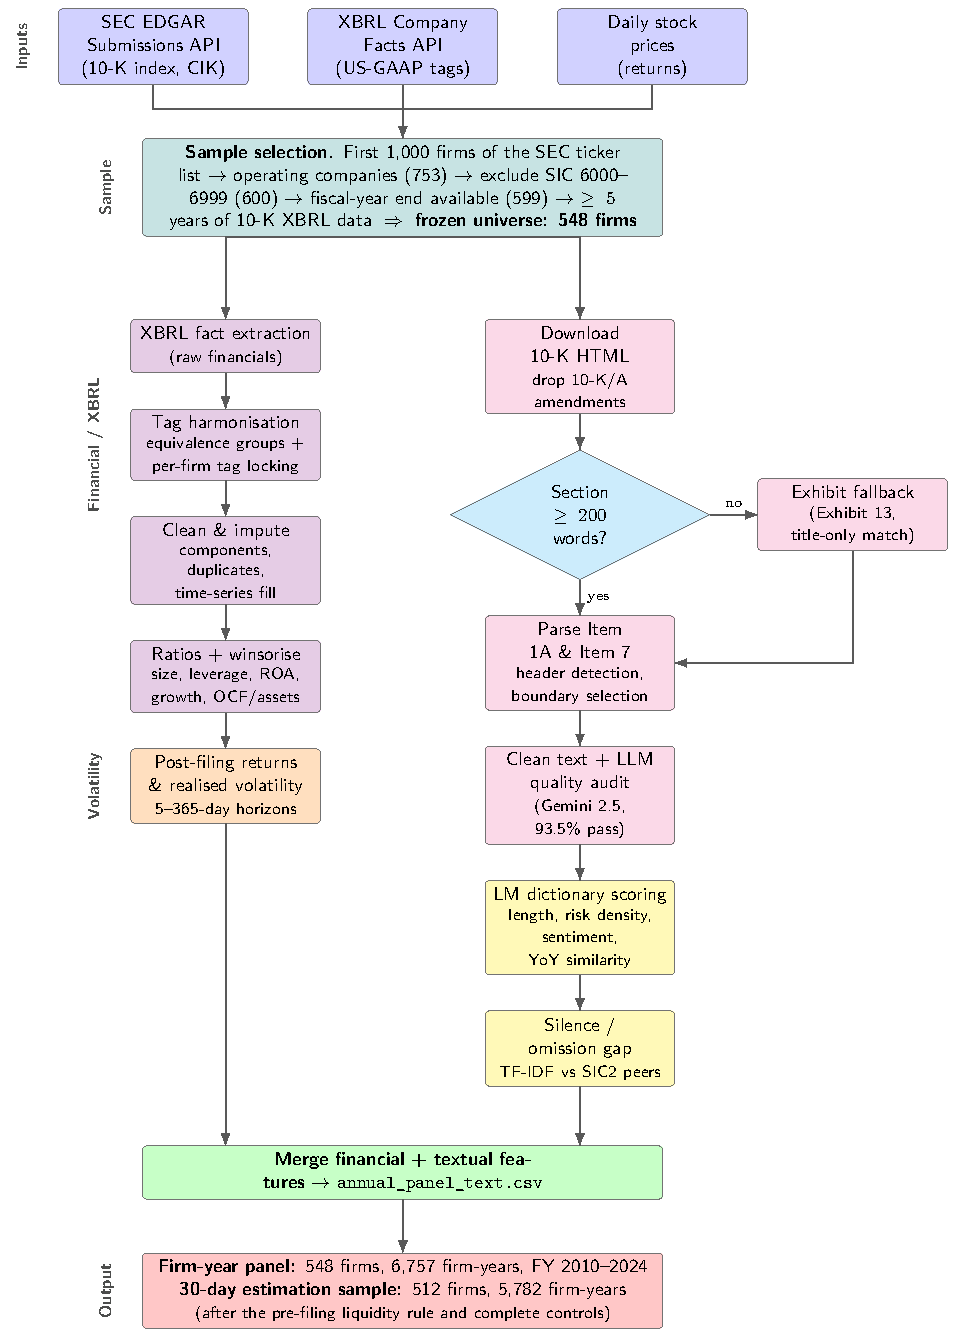
\includegraphics[width=\textwidth]{img/fig_data_pipeline.pdf}
\caption{Operational pipeline for the complete data preparation.
The workflow runs top-to-bottom from the raw SEC sources through sample
selection, then splits into a financial (XBRL) branch and a textual
(10-K narrative) branch that are merged into the final regression-ready
firm-year panel. Own processing.}
\label{fig:data_pipeline}
\end{figure}


% ─────────────────────────────────────────────────────────────────────────────
\section{Sample selection}
\label{sec:sample_selection}
% ─────────────────────────────────────────────────────────────────────────────

The starting universe is the first 1{,}000 entries in the SEC file
\texttt{company\_tickers.json}, which maps stock tickers to Central Index Keys
(CIKs). The version used in this study was archived in the project repository
in October 2026. Three filters are then applied (Table~\ref{tab:attrition} in
Appendix~\ref{app:variables}). First, only entities classified by the SEC as
operating companies are retained, which excludes exchange-traded funds,
closed-end funds, and shell companies (1{,}000 to 753). Second, firms with SIC
codes 6000--6999 (finance, insurance, and real estate) are excluded. Following
\textcite{fama1992}, financial firms are omitted because leverage and related
balance-sheet ratios have a different economic interpretation for such firms
than for non-financial operating companies, as financial assets and
liabilities constitute a core component of their business model rather than
primarily a financing choice. This filter reduces the sample from 753 to 600
firms. Third, firms must have at least five fiscal years of available 10-K
XBRL data. This requirement ensures that lagged variables, such as asset
growth, can be constructed while still leaving at least four years of usable
panel observations. The filter reduces the sample to 550 firms using current
metadata; the frozen sample used in the final analysis contains 548 firms.

Earlier versions of this panel also dropped firms with valid post-filing
volatility for fewer than 90\% of their filings. That filter used prices
\emph{after} each filing, that is, it selected on the outcome period, and it
has been removed. Instead, a filing enters the regressions only if the stock
has at least 200 daily closing prices in the 252 trading days \emph{before}
the filing date; this removes thinly traded or newly listed stocks using
information available at the filing date and affects 1.3\% of filings.

\paragraph{Sample size and look-ahead.} Large firms have complete
machine-readable filing histories, are liquid, and their filings are
consistently formatted, which keeps measurement error in both branches low.
The cost is that the list is drawn from today's large firms: firms that
failed, were acquired or shrank during 2010--2024 are missing, and the panel
grows from 152 firm-years in fiscal year 2010 to over 500 from 2020. The
results therefore describe large surviving U.S.\ firms
(Section~\ref{sec:estimation}). The 30-day estimation sample has 5{,}782
firm-years of 512 firms. By comparison, \textcite{campbell2014} study
risk-factor disclosures of a broad cross-section of U.S.\ firms and
\textcite{loughran2011} use about 50{,}000 10-K filings; their aims require
broad coverage, whereas the within-industry-year comparisons here rely on a
balanced set of large issuers. % TODO verify: Campbell et al. (2014) sample size (#9)


% ─────────────────────────────────────────────────────────────────────────────
\section{Annual filings as the unit of observation}
\label{sec:annual_vs_quarterly}
% ─────────────────────────────────────────────────────────────────────────────

We use annual 10-K filings rather than quarterly 10-Q reports. A quarterly
panel would have roughly four times as many observations, but two problems
appeared in small pilot tests (Tables~\ref{tab:q4_reliability}
and~\ref{tab:text_availability}); the pilots are illustrations on a handful
of firms, not representative estimates.

\paragraph{Financial data in the fourth quarter.} 10-Q filings cover only the
first three quarters, so a quarterly panel must reconstruct the fourth
quarter as the annual figure minus the three quarters. In a pilot of 30
non-financial firms (Table~\ref{tab:q4_reliability}), all three quarterly
operating-cash-flow facts were available in only 7\% of firm-years, because
most firms report cumulative year-to-date cash flows. Operating cash flow
enters the control vector, so a quarterly panel would lose it at the source.
For net income and operating income the implied and the explicitly reported
fourth quarter differ by more than 1\% of the annual figure in about 10 to
14\% of comparable firm-years. The residual absorbs year-end audit
adjustments that are booked in the fourth quarter, whereas a later filing may
report a recast figure, so the two represent different versions of the same
accounting history.

\begin{table}[htbp]
\centering
\caption{Q4 Reliability: Availability and Consistency of Fourth-Quarter XBRL Facts}
\label{tab:q4_reliability}
\small
\setlength{\tabcolsep}{5pt}
\begin{tabular}{lrrrrr}
\toprule
Metric & Firm-Years & Q1\,--\,Q3 (\%) & Explicit Q4 (\%) & Comparable & Match (\%) \\
\midrule
Net Income & 451 & 80.9 & 43.0 & 172 & 89.5 \\
Operating Income & 391 & 79.0 & 22.0 & 72 & 86.1 \\
Operating Cash Flow & 462 & 7.4 & 3.2 & 0 & --- \\
\bottomrule
\end{tabular}
\begin{tablenotes}
\small
\item \textit{Note:} ``Q1\,--\,Q3'' indicates the share of fiscal years where all three
quarterly facts (Q1, Q2, Q3) exist in XBRL. ``Explicit Q4'' indicates the share with
a standalone fourth-quarter fact (period $\approx$90~days ending at fiscal year-end).
``Comparable'' is the count of firm-years for which both an explicit Q4 fact and the
implied residual are available. ``Match'' reports the share of those comparable
observations where the two values agree within 1\% of the annual figure.
Sample: 30 non-financial firms, all available fiscal years.
\end{tablenotes}
\end{table}


\paragraph{Risk factors in quarterly reports.} Form 10-Q (Part~II, Item~1A)
requires only \emph{material changes} to the risk factors disclosed in the
latest 10-K, whose content is governed by Item~105 of Regulation S-K
(17~CFR~229.105). In a pilot of the six most recent 10-Q filings of 15 large
firms, 52\% contained a substantive risk-factor section and the rest referred
back to the annual report (Table~\ref{tab:text_availability};
Table~\ref{tab:text_per_company} lists the firms). Text variables measured
on the full risk-factor section therefore cannot be built quarterly.

\begin{table}[htbp]
\centering
\caption{Textual Data Availability: 10-K vs.\ 10-Q Filings}
\label{tab:text_availability}
\begin{tabular}{lrr}
\toprule
 & 10-K & 10-Q \\
\midrule
Filings tested & 44 & 90 \\
\addlinespace
\multicolumn{3}{l}{\textit{MD\&A (Management's Discussion and Analysis)}} \\
\quad Section found (\%) & 93 & 100 \\
\quad Median word count & 20,494 & 5,806 \\
\addlinespace
\multicolumn{3}{l}{\textit{Risk Factors}} \\
\quad Substantive section found (\%) & 100 & 52 \\
\quad Boilerplate / reference only (\%) & 0 & 48 \\
\quad Median word count (substantive) & 29,902 & 9,144 \\
\bottomrule
\end{tabular}
\begin{tablenotes}
\small
\item \textit{Note:} ``Found'' requires $>$200 words extracted by regex-based section
parser. ``Substantive'' for 10-Q excludes filings containing only a reference to the
annual 10-K (e.g., ``no material changes from those disclosed in our Annual Report'').
MD\&A corresponds to Item~7 in 10-K and Part~I Item~2 in 10-Q; Risk Factors
corresponds to Item~1A in 10-K and Part~II Item~1A in 10-Q.
Sample: 15 firms, most recent filings.
\end{tablenotes}
\end{table}


Annual filings contain audited full-year accounting data and complete
risk-factor and MD\&A sections, and they are the unit of analysis in the
10-K textual-analysis literature \parencite{li2008, loughran2011}. Matching
the observation interval to the reporting frequency of the documents also
means that changes in the text variables correspond to actual revisions of
the annual disclosure.


% ─────────────────────────────────────────────────────────────────────────────
\section{Financial data from XBRL}
\label{sec:xbrl_tags}
% ─────────────────────────────────────────────────────────────────────────────

\paragraph{Point-in-time values.} For each firm and fiscal period the panel
takes the values, the filing date and the accession number of the
\emph{first} 10-K that reports facts for that period end, filed within 180
days of it. Restated figures published later (in a 10-K/A or as comparatives
in the next year's 10-K) are not mixed in, because they were not public when
the post-filing window starts. A 10-K/A is used only when no original 10-K
reports the period. All variables of a firm-year therefore come from one
filing, identified by its accession number, which also identifies the
filing whose text is used. The fiscal year is the calendar year in which the
period ends (periods ending on 1--7 January count to the previous year, for
firms with 52/53-week years).

\paragraph{Fiscal years and calendar time.} Firms do not share a fiscal
calendar, so the 10-Ks of one fiscal year are filed at different calendar
dates (Table~\ref{tab:timing} in Appendix~\ref{app:variables}). 72.6\% of the
firm-years end in December, and 145 of the 512 firms in the estimation sample
have a different fiscal-year end, from January to November. The median lag
between period end and filing is 53 days (10th to 90th percentile: 38 to 59
days), so most filings fall in February, but the filings of one fiscal year
span a median of 390 calendar days and fall in 169 distinct calendar months.
Four choices keep this heterogeneity from distorting the analysis. First, the
fiscal year is assigned from the period end itself, not from the fiscal-year
end month that the SEC reports today, which is unreliable for firms with
52/53-week years and had shifted the labels of about 20 firms by one year in
an earlier version of the panel. Second, every timing variable is anchored on
the firm's own filing date, not on a common calendar date: the outcome
window, the pre-filing windows and the lagged volatility of the previous
filing all start at that firm's day~0 (Section~\ref{sec:outcome}), and the
accounting variables and the text come from the filing that opens the window.
Third, the previous fiscal year is matched only when it is exactly one year
earlier, so that a change of the fiscal-year end never produces a lag of
unequal length. Fourth, because a fiscal-year effect cannot remove
calendar-time shocks when the filings of one fiscal year are spread over more
than a year, the robustness checks replace it by the calendar month of the
filing and restrict the sample to firms with a December year end
(Section~\ref{sec:robustness_h12}).

\paragraph{Tag choices.} One accounting concept can be reported under several
US-GAAP elements, so the elements must be mapped explicitly
\parencite{chychyla2015}. Two kinds of alternatives are handled differently.
\begin{itemize}
  \item \emph{Equivalent tags} measure the same quantity and are used
    interchangeably. Net income is measured on a consolidated basis:
    \texttt{ProfitLoss} (including non-controlling interests, NCI) where a
    firm reports it, and \texttt{NetIncomeLoss} otherwise, which under
    US GAAP is then the same consolidated figure. This makes ROA consistent
    with total assets and total liabilities, which also include NCI. The two
    operating-cash-flow tags (total and continuing operations) are also
    treated as equivalent.
  \item \emph{Non-equivalent tags}, such as stockholders' equity with or
    without NCI, or income from continuing operations versus net income, are
    \emph{locked} per firm: each firm keeps the tag it reports in most years,
    and values under other tags are set to missing. The choice uses the
    firm's whole history, a mild look-ahead in which tag is used, not in the
    values.
\end{itemize}

Table~\ref{tab:tag_provenance} in Appendix~\ref{app:variables} reports the
tag choices, the values lost to locking (637 of 7{,}900 equity values, 38
net-income values, no cash-flow values) and the differences between paired
tags in firm-years that report both. Where both net-income tags are present
(3{,}838 firm-years), the median absolute difference is 0.043\% of total
assets, but the 99th percentile is 3.56\% and the maximum 37.4\%; in 303
firm-years (7.9\%) the difference exceeds 1\% of total assets, which we call
material. These differences are the NCI share of income, which the
consolidated definition now includes consistently. For the two
operating-cash-flow tags (417 firm-years) the difference exceeds 1\% of
assets in 50 firm-years (12.0\%), with a median of 0.035\%.

\paragraph{Missing balance-sheet values.} If total liabilities are missing,
they are computed as total assets minus stockholders' equity (2{,}171
firm-years). If total assets or liabilities are still missing, the value of
the immediately preceding fiscal year is carried forward (1 and 32
firm-years); values are never filled from later years. Each imputation is
flagged, and Section~\ref{sec:robustness_h12} re-estimates the models without
imputed values.

\paragraph{Market capitalisation.} Shares outstanding are taken from the same
10-K as the other variables, matched by accession number: the cover-page
count (\texttt{dei:EntityCommonStockSharesOutstanding}, summed over share
classes), else the balance-sheet count, else the fiscal-year weighted-average
basic count. The last source is needed for multi-class firms whose
cover-page counts are reported per class and are not available in the
Company Facts API (445 firm-years); a robustness check drops these
firm-years. Shares are multiplied by the as-traded closing price on the last
trading day before the filing, which is rebuilt from the split-adjusted
price and the split history.


% ─────────────────────────────────────────────────────────────────────────────
\section{Text extraction from 10-K filings}
\label{sec:text_extraction}
% ─────────────────────────────────────────────────────────────────────────────

The study uses Item~1A (Risk Factors) and Item~7 (Management's Discussion
and Analysis, MD\&A) of the 10-K.

\subsection{Source of the text}
\label{ssec:text_source}

For each original 10-K in the panel the primary HTML document was downloaded
from the EDGAR archive, using the document name listed in the EDGAR
Submissions API.\footnote{%
\texttt{https://data.sec.gov/submissions/CIK\{cik\}.json}; see
\url{https://www.sec.gov/search-filings/edgar-application-programming-interfaces}.}
Where the filing incorporates a section by reference to an exhibit, the
exhibit was fetched from the same filing (Section~\ref{ssec:section_id}).
All requests carried the declared user-agent header that the SEC requires
and stayed below its limit of ten requests per second. The extraction was
run once, in October 2026; the stored texts were not re-extracted for this
version, and each stored section is linked to the accession number of the
filing it came from. In seven firm-years the stored text comes from a 10-K/A
whereas the panel now uses the original 10-K; these firm-years are excluded
from all text regressions.

\subsection{Section identification and exhibit fallback}
\label{ssec:section_id}

The text of a 10-K is embedded in HTML without standard tagging, mixed with
table-of-contents entries, running headers and cross-references, so a plain
search for ``Item~1A'' typically finds the table of contents. The parser
works on the document structure before the text is flattened:
\begin{enumerate}
  \item \textbf{Candidate detection.} Elements (paragraphs, divisions, table
    cells, headings) whose text matches an ``Item~X'' pattern are kept as
    candidate headers if they have at most 25 words, carry a heading cue
    (bold font, all capitals, or a font size of at least 12\,pt), and contain
    no hyperlink (table-of-contents links).
  \item \textbf{In-place tagging.} Each candidate is marked inside the HTML
    tree, and only then is the document converted to text, so header
    positions survive the conversion.
  \item \textbf{Candidate selection.} A candidate for Item~1A must have the
    word ``risk'' within 300 characters, and one for Item~7 ``management'',
    ``discussion'' or ``MD\&A''. Candidates with at least three other item
    headers within 300 characters (a table of contents) and candidates
    preceded by ``see'', ``refer to'' or similar phrases are discarded when
    alternatives exist. Among the rest the parser takes the candidate
    followed by the longest section.
  \item \textbf{Section bounding.} The section ends at the next item header:
    Item~1B, 1C or 2 for Item~1A, and Item~7A, 8, 9, 9A or 9B for Item~7.
    Several terminators are needed because some items are optional (Item~1B
    applies only to some filers, and Item~1C exists only for fiscal years
    ending on or after 15~December~2023). A section needs at least 200 words.
\end{enumerate}

\paragraph{Exhibit fallback.} Some filers, especially early in the sample,
incorporate the MD\&A by reference to the annual report to shareholders,
attached as an exhibit (usually Exhibit~13). If no section of at least 200
words is found and the text under the header (fewer than 500 words) refers
to an exhibit or the annual report, the parser applies the same procedure to
the referenced exhibit, using title patterns (``Risk Factors'',
``Management's Discussion and Analysis'') because exhibits have no item
numbers. The extraction run did not record which sections came from an
exhibit, and the share cannot be measured without downloading the filings
again. We expect it to be small and concentrated in Item~7 of early years:
Item~1A must appear in the body of the 10-K itself, and incorporation by
reference to the annual report was mainly used for MD\&A.

\subsection{Post-processing and tokenisation}
\label{ssec:text_postprocessing}

During the HTML conversion, scripts, style sheets and the hidden inline-XBRL
header are removed, and tables are removed if they are numerical: at least
30\% of their non-empty cells (with at least four cells and two rows) are
bare numbers or currency amounts, or more than 40\% of their characters are
digits or number symbols. Other tables, which in many filings are used for
page layout, keep their text. After the section has been bounded, the parser
removes running ``Table of Contents'' headers, page footers such as ``2019
Form 10-K 59'', standalone page numbers, residual numeric table rows (lines
of at least four tokens of which more than 40\% are numbers), and short lines
that repeat at least four times (running headers), and replaces non-breaking
spaces. Footnote markers and text of layout tables are not removed.

For the dictionary measures the text is lowercased and split into tokens of
at least two letters (digits, hyphens and apostrophes split tokens); a
section with fewer than 100 tokens is treated as missing. The dictionary is
the Loughran--McDonald Master Dictionary, 1993--2025 version
\parencite{loughran2011}, with 297 uncertainty and 903 litigious words; words
that the dictionary marks as removed are not counted. The two lists share
no word.

\subsection{Coverage}
\label{ssec:text_coverage}

Of the 6{,}757 firm-years of the panel, 96.3\% have an Item~1A of at least
100 tokens and 94.9\% an Item~7 (Table~\ref{tab:text_coverage} in
Appendix~\ref{app:variables}). Coverage is lowest in fiscal year 2010
(92.8\%) and is 94.7\% in 2024; the lower 2024 figure comes from a correction
of the fiscal-year labels of about 15 firms with 52/53-week years, whose
fiscal-year-2024 filing had not been extracted.

\paragraph{Extraction audits.} Two large language models (LLMs) audited a
stratified random sample of stored sections. The sample has five three-year
strata (2010--2012 to 2022--2024) with 20 sections of each type per stratum,
200 sections in total; Item~1A and Item~7 were drawn independently, so the
200 sections come from 197 filings. Each section was rated on five criteria
(correct section, start boundary, end boundary, content quality,
completeness) as Pass, Minor issue or Fail. The first audit, by Google
Gemini~2.5~Flash, saw the full extracted section; a second, independent
audit by Claude Opus~5.5 saw the first and last 1{,}200 characters, a middle
excerpt and the word count, without the first audit's ratings. Neither saw
the rest of the filing, so boundary judgements rest on the extracted text
alone. LLMs perform well on text-classification tasks compared with crowd
workers \parencite{gilardi2023}, but their judgements are not a substitute
for an expert reading of the filings. The author therefore also checked 51
of the sections by hand against the original filings on EDGAR, without
seeing the LLM ratings: 50 drawn at random within the same strata and the
one further section flagged by an LLM.

Under the first audit, 187 of 200 sections (93.5\%, Wilson 95\% interval
89.2--96.2\%) were acceptable on all five criteria (Pass or Minor) and 179
(89.5\%) were rated Pass on all five. The 13 sections with a Fail include five
with no extracted text; by stratum, five fall in 2010--2012, three in
2013--2015, two each in 2016--2018 and 2019--2021, and one in 2022--2024.
Under the second audit 190 sections (95.0\%, 91.0--97.3\%) were acceptable;
the two audits agree on 96.5\% of sections ($\kappa = 0.68$) and both reject
the same eight (Table~\ref{tab:ai_validation} in Appendix~\ref{app:ai-usage}).
In the manual check every one of the 51 sections was the correct section;
four had a boundary error (two started inside Item~1, one ran a few lines into the
financial statements and one ran through Item~8), three of them among the
50 random sections, an error rate of 6.0\% (Wilson 95\% interval
2.1--16.2\%). The manual verdict on the three criteria matches the first
audit on all 51 sections and the second on 50.
Errors are more frequent in early filings, whose structure is less
standardised.

\paragraph{Relation to other approaches.} Changes in the structure of 10-K
filings over time make large-sample extraction difficult
\parencite{dyer2017}. Sections tagged in XBRL (for example
\texttt{us-gaap:RiskFactorsTextBlock}) are incomplete and inconsistent in
early years, so a parser that works on the HTML lets the same method be
applied to the whole 2010--2024 period.

% =============================================================================
\chapter{Methodology}
\label{ch:methodology}
% =============================================================================

This chapter describes the regressions I use to test the three hypotheses.
In every test, I regress post-filing realised volatility on features of the
Item~1A risk-factor section, a common set of controls that are known when the
10-K is filed, and fixed effects.
Section~\ref{sec:outcome} defines the dependent variable and explains when
each variable is measured. Section~\ref{sec:controls} lists the controls. They
are the same in every specification, so the text coefficients can be compared
across hypotheses. Sections~\ref{sec:h1} and~\ref{sec:h2} cover the joint
test of the volume channel (H1) and the composition channel (H2). I estimate
them together because the density measure for H2 has section length in its
denominator. Section~\ref{sec:h3} introduces the peer-relative omission gap
for H3 and the decision rule I use to judge it. Section~\ref{sec:estimation}
covers estimation and inference.


% ─────────────────────────────────────────────────────────────────────────────
\section{Outcome variable and timing}
\label{sec:outcome}
% ─────────────────────────────────────────────────────────────────────────────

The dependent variable is the natural logarithm of annualised post-filing
stock-return volatility measured over a window of $h$~calendar days:
\begin{equation}
\ln \sigma_{i,t+1}^{[h]} \;=\; \ln\!\left(
\sqrt{252}\cdot
\operatorname{sd}\!\bigl(r_{i,d}\bigr)_{d \in W_{i,t}^{[h]}}
\right),
\label{eq:vol}
\end{equation}
where $r_{i,d} = \ln(P_{i,d}/P_{i,d-1})$ is the daily log return of firm~$i$
computed from dividend- and split-adjusted closing prices, and
$W_{i,t}^{[h]}$ is the post-filing window that belongs to the 10-K for fiscal
year~$t$. The subscript $t+1$ only means that the window comes after the
filing; it does not refer to the next fiscal year. Day~0 is the first trading
day on or after the filing date. The window starts two trading days after
day~0, so the market reaction on the filing day and the day after is left
out, and it then runs for $h$~calendar days. Only returns between two prices
inside the window are used. A window needs a minimum number of daily returns
(3 for $h = 5$, 5 for $h = 10$, 14 for $h = 30$, and 44, 89 and 199 for the
longer windows). If there are fewer, or if the standard deviation is zero,
the volatility is treated as missing. A window that would end after the last
trading day in the price data (30~October 2026) is also treated as missing
instead of being cut short. With this cut-off, every fiscal-year~2024 filing
has a complete 365-day window (Section~\ref{sec:sample_selection}).

Figure~\ref{fig:timeline} shows the timing. Every control and every text
variable uses only information that is public at day~0. The accounting
variables and the text come from the same 10-K, and the price-based controls
use windows that end on the last trading day before the filing date.

\begin{figure}[htbp]
\centering
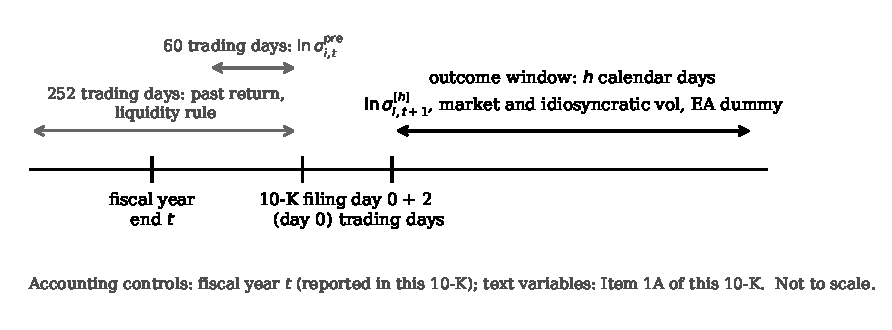
\includegraphics[width=\textwidth]{img/fig_timeline.pdf}
\caption{Timing of the variables for the 10-K of fiscal year $t$ (not to
scale). The outcome window starts two trading days after day~0 and lasts
$h$ calendar days; pre-filing volatility uses the 60 trading days, and the
past return and the liquidity rule the 252 trading days, that end on the
last trading day before the filing date.}
\label{fig:timeline}
\end{figure}

A coefficient $\beta$ on a regressor $x$ means that volatility changes by
$100(e^{\beta\Delta x}-1)\%$ when $x$ changes by $\Delta x$. The main horizon
is $h = 30$ calendar days. I chose it to keep the outcome close to the filing,
so that later news has less time to affect it. Earlier studies that link 10-K
text to later stock-return volatility have used windows of about one year
\parencite{campbell2014, kogan2009, loughran2011}. I report the 365-day window
alongside the main result and use $h \in \{5, 10, 90, 180\}$ as robustness
checks.


% ─────────────────────────────────────────────────────────────────────────────
\section{Control variables}
\label{sec:controls}
% ─────────────────────────────────────────────────────────────────────────────

Every regression for H1, H2 and H3 includes the same vector
$\mathbf{X}_{i,t}$ of nine controls. All of them are known at day~0:
\begin{itemize}
  \item pre-filing volatility $\ln\sigma^{\mathrm{pre}}_{i,t}$: the log of the
    annualised standard deviation of the 60 daily returns ending on the last
    trading day before the filing date;
  \item firm size $\ln(\text{Market cap})$: the as-traded closing price on the
    last trading day before filing times the shares outstanding reported in
    the same 10-K;
  \item book-to-market: book equity attributable to the parent over market
    capitalisation (total equity including NCI where parent equity is not
    reported; Section~\ref{sec:xbrl_tags});
  \item the past 12-month log return, over the 252 trading days before filing;
  \item leverage (total liabilities over total assets), return on assets
    (consolidated net income over total assets), asset growth, the current
    ratio, and operating cash flow over total assets.
\end{itemize}
Pre-filing volatility is the most important control. Stock-return volatility
is persistent \parencite{kogan2009}, and the way a firm writes its disclosure
may reflect conditions that were already visible before the filing. Firm size,
book-to-market, past returns and leverage also appear in earlier
risk-disclosure regressions \parencite{campbell2014}, although the variables
are defined differently. The remaining accounting ratios control for
profitability, growth, liquidity and operating cash flow. Operating cash flow
over assets is part of the main specifications and not only a robustness
check.

An earlier version of this model used a different dynamic control: the
volatility of a window of the same length after the previous year's 10-K.
Once pre-filing volatility is included, this lag adds nothing. Its
coefficient is $+0.031$ with $t=+0.69$ in the industry fixed-effects model
(Table~\ref{tab:firm_fe} reports the firm fixed-effects version), so I report
it only as a robustness check. Each firm's first fiscal year is not in the
sample, because asset growth needs the previous year's total assets.
Financial ratios, book-to-market and the past return are winsorised at the
1st and 99th percentiles of each regression sample. Market capitalisation and
pre-filing volatility enter in logs and are not winsorised.


% ─────────────────────────────────────────────────────────────────────────────
\section{H1 --- Item~1A length and disclosure volume}
\label{sec:h1}
% ─────────────────────────────────────────────────────────────────────────────

Following \textcite{campbell2014}, I measure disclosure volume as the
logarithm of the Item~1A word count. Campbell et al.\ find that firms with
longer risk-factor sections have higher market-based risk measures later on.
This fits the idea that the amount of risk discussion carries information
about the firm's risk. The volume variable is
\begin{equation}
\text{Words}^{1A}_{i,t} \;=\; \text{number of tokens in Item~1A of firm
$i$'s fiscal-year-$t$ 10-K},
\end{equation}
where a token is a run of at least two letters in the lowercased text
(Section~\ref{ssec:text_postprocessing}). The cleaning removes running
page headers, page numbers and numeric table rows. It keeps the text of
layout tables and footnote markers, so the count is close to the narrative
content but not identical to it. The median Item~1A in the estimation sample
has 8{,}700 tokens (Table~\ref{tab:summary}).

\paragraph{H1.} \emph{If the composition of Item~1A and the controls are held
fixed, a longer Item~1A is associated with higher post-filing volatility}:
$\beta^{\text{len}} > 0$ in
\begin{multline}
\ln \sigma_{i,t+1}^{[h]} \;=\; \alpha
\;+\; \boldsymbol{\gamma}' \mathbf{X}_{i,t}
\;+\; \beta^{\text{len}} \ln(\text{Words}^{1A}_{i,t}) \\
\;+\; \beta^{\text{dens}} \,\text{RiskDensity}_{i,t}
\;+\; \mu_{j(i,t)} \;+\; \tau_t
\;+\; \varepsilon_{i,t},
\label{eq:joint_model}
\end{multline}
where $\mu_j$ is a fixed effect for the two-digit SIC industry of the firm at
the filing date, $\tau_t$ is a fiscal-year fixed effect, and RiskDensity is
defined in Section~\ref{sec:h2}. Length and density enter together because
length is in the denominator of the density.


% ─────────────────────────────────────────────────────────────────────────────
\section{H2 --- Risk-word density}
\label{sec:h2}
% ─────────────────────────────────────────────────────────────────────────────

H2 is about the composition of Item~1A at a given length. It uses the share of
words from the uncertainty and litigious dictionaries of
\textcite{loughran2011}, which were built for financial reporting:
\begin{equation}
\text{RiskDensity}_{i,t} \;=\; \frac{n^{\text{unc}}_{i,t} + n^{\text{lit}}_{i,t}}
{\text{Words}^{1A}_{i,t}},
\label{eq:risk_density}
\end{equation}
where $n^{\text{unc}}$ and $n^{\text{lit}}$ count the tokens of Item~1A that
belong to each list. The two lists share no word in the dictionary version I
use (Section~\ref{ssec:text_postprocessing}), so no token is counted twice.

Previous studies do not give a clear prediction for how this density measure
relates to volatility, so H2 is two-sided. I consider two possible
explanations.

\textbf{Risk content.} Uncertainty and litigious words may describe uncertain
outcomes and legal risks. \textcite{campbell2014} find that risk-factor
disclosures reflect the risks firms face, and \textcite{kravet2013} find that
increases in risk disclosure go together with increases in stock-return
volatility. If a higher density of risk words means the section says more
about risk, it should be associated with higher volatility.

\textbf{Standard language.} Risk disclosures may also contain general
language that firms repeat or copy. \textcite{cazier2021} show that firms have
reasons to use standard risk language and sometimes borrow it from other
firms. \textcite{dyer2017} document repetition and boilerplate in 10-K
reports, and \textcite{hope2016} find that more specific risk disclosures are
useful to investors and analysts. A high share of risk words may therefore
reflect standard wording and not real information about the firm's risks.
This could weaken the link between risk-word density and volatility, but it
does not by itself predict lower volatility.

\paragraph{H2.} If Item 1A length and the other controls are held fixed,
RiskDensity is associated with post-filing volatility: $(\beta_{\mathrm{dens}}\neq 0)$ in equation~(3.3). The sign shows the direction of the association, but it does not tell us which channel is behind it. Density measures the share of selected words, not how specific the disclosure is, which is what \textcite{hope2016} study. Words such as ``litigation'' or ``investigation'' can also appear in descriptions of very specific events.

\paragraph{Sub-list decomposition.} A second specification replaces
RiskDensity with its two components:
\[
\mathrm{UncDensity}_{i,t} = \frac{n^{\mathrm{unc}}_{i,t}}{\mathrm{Words1A}_{i,t}},
\qquad
\mathrm{LitDensity}_{i,t} = \frac{n^{\mathrm{lit}}_{i,t}}{\mathrm{Words1A}_{i,t}}.
\]
\begin{align}
\ln \sigma_{i,t+1}^{[h]}
&= \alpha + \gamma' X_{i,t}
+ \beta_{\mathrm{len}} \ln(\mathrm{Words1A}_{i,t})
+ \beta_{\mathrm{unc}} \mathrm{UncDensity}_{i,t}
+ \beta_{\mathrm{lit}} \mathrm{LitDensity}_{i,t}
+ \mu_{j(i,t)} + \tau_t + \varepsilon_{i,t}.
\label{eq:decomposition_model}
\tag{3.5}
\end{align}
The uncertainty list captures uncertain and imprecise wording. The litigious list captures legal and regulatory language, which does not always point to an actual legal dispute or exposure \parencite{loughran2011}. A Wald test of $(\beta_{\mathrm{unc}} = \beta_{\mathrm{lit}})$ checks whether the two densities are associated differently with volatility.

\paragraph{Ratio regressors.} Both densities divide word counts by Item 1A
length. Ratios can give misleading results if the role of the denominator is
not handled carefully \parencite{kronmal1993}. The model includes log length to
account for differences in section length, but this does not guarantee that
the problem goes away. As a robustness check, I replace the densities with
$(\ln(1+n^{\mathrm{unc}}))$ and $(\ln(1+n^{\mathrm{lit}}))$ and keep
$\ln(\mathrm{Words1A})$ (Section~\ref{sec:robustness_h12}). This model uses
counts that are not divided by length. Comparing the two sets of results shows
whether the findings depend on how risk language is measured.


% ─────────────────────────────────────────────────────────────────────────────
\section{H3 --- Peer-relative omission gap}
\label{sec:h3}
% ─────────────────────────────────────────────────────────────────────────────

H3 asks whether the topics a firm \emph{leaves out} of Item~1A, compared with
its industry peers, help predict later volatility once length and density are
accounted for. I call this measure the \emph{omission gap}. One way to read it
is as \emph{strategic silence}: the firm says little about risks that its
peers discuss. But other explanations would produce the same pattern. The
firm may simply not face that risk, may use different words for it, or may
write a shorter section for reasons unrelated to risk.

\paragraph{Construction.} For each fiscal year $t$, I fit a TF--IDF model on
the Item~1A texts filed before the first fiscal-year-$t$ filing in the panel.
This way, the vocabulary and weights are already known on the date of every
filing I analyse (fiscal year 2010 has no earlier texts, so it has no omission
gap). I use the standard \texttt{scikit-learn} Python library for the text
vectorisation, with these settings: the text is lowercased; tokens must have
at least two letters or digits; the library's English stop-word list is
removed; only single words are used; a term must appear in at least five
documents and in at most 95\% of the training documents; raw term counts are
used; inverse document frequency is smoothed; and each row is scaled to
unit length. Let $\mathbf{x}_{i,t}$ be the TF--IDF row of firm $i$'s
fiscal-year-$t$ Item~1A. The peers of a filing are the other panel firms in the
same two-digit SIC industry (at the filing date). For each peer, I use the
most recent Item~1A from fiscal year $t$ or $t-1$ that was filed strictly
before the focal filing, so no later information is used. With $P_{i,t}$ as
this peer set,
\begin{equation}
\mathbf{p}_{i,t} = \sum_{k \in P_{i,t}} \mathbf{x}_{k},
\qquad
\textsc{Omission}^{1A}_{i,t} \;=\; 1 \;-\;
  \frac{\sum_{w : x_{i,t,w} > 0}\, p_{i,t,w}}{\sum_{w}\, p_{i,t,w}},
\label{eq:omission}
\end{equation}
the share of peer TF--IDF weight that falls on terms the focal firm does not
use. It lies between 0 and 1. Filings with fewer than five peers get no value.

\paragraph{Length and the sources of variation.} The omission gap is closely
tied to length, because a longer section naturally covers more of the peer
vocabulary. In the H3 sample, its correlation with $\ln(\text{Words}^{1A})$ is
$-0.915$ (Table~\ref{tab:silence_diag}). To deal with this, and to see where
the variation in the gap comes from, I use three variants:
\begin{itemize}
  \item a \emph{length-invariant} omission gap. For each filing, I draw 20
    random blocks of 3{,}000 consecutive tokens from its Item~1A (with a fixed
    seed), compute the gap on each block instead of the full text, and
    average the 20 values. Sections shorter than 3{,}000 tokens use the whole
    text;
  \item a \emph{pooled-vocabulary} gap, using one TF--IDF model fitted on all
    years. This removes changes in vocabulary over time. Because it uses
    later documents, I use it only as a diagnostic;
  \item a breakdown of the year-on-year change in the gap into three
    parts: the change in the firm's own text (with peers held at $t-1$), the
    change in the peers' texts, and the change in who the peers are.
\end{itemize}

\paragraph{Specification.} The H3 regression adds the omission gap to
equation~\eqref{eq:joint_model}:
\begin{multline}
\ln \sigma_{i,t+1}^{[h]} \;=\; \alpha
\;+\; \boldsymbol{\gamma}' \mathbf{X}_{i,t}
\;+\; \beta^{\text{len}} \ln(\text{Words}^{1A}_{i,t})
\;+\; \beta^{\text{dens}} \,\text{RiskDensity}_{i,t} \\
\;+\; \beta^{\text{om}} \,\textsc{Omission}^{1A}_{i,t}
\;+\; \mu \;+\; \tau_t
\;+\; \varepsilon_{i,t},
\label{eq:silence_model}
\end{multline}
I estimate it with industry fixed effects ($\mu = \mu_j$) and with firm fixed
effects ($\mu = \mu_i$). The controls are the same as in
Section~\ref{sec:controls}, so the H3 model differs from the H1/H2 model
only by the omission gap.

\paragraph{H3 and the decision rule.} \emph{If length, density and the
controls are held fixed, a larger omission gap is associated with higher
post-filing volatility}, that is, $\beta^{\text{om}} > 0$. I judge the
evidence with a fixed rule, which I wrote down in the project log before
re-estimating the models:
\begin{enumerate}
  \item The family of tests covers $h \in \{5, 10, 30, 90, 180\}$ days under
    both fixed-effect structures, which gives ten two-sided tests. I adjust
    the $p$-values with the Holm step-down procedure \parencite{holm1979} at
    $\alpha = 0.05$.
  \item The primary design is $h = 30$ days. Under a given fixed-effect
    structure, there is \emph{positive evidence} if $\beta^{\text{om}} > 0$
    with Holm-adjusted $p < 0.05$ \emph{and} the length-invariant gap also has
    a positive coefficient with $p < 0.05$ in the same specification.
    \emph{Negative evidence} is the mirror image.
  \item H3 is \emph{supported} if there is positive evidence under both
    structures. It is \emph{partially supported} if there is positive evidence
    under one and no negative evidence under the other. It is
    \emph{contradicted} if there is only negative evidence, and
    \emph{not supported} in all other cases. Both fixed-effect structures
    are treated the same way.
\end{enumerate}
I report the placebo test, the decomposition and the other robustness checks,
but they do not change the verdict.


% ─────────────────────────────────────────────────────────────────────────────
\section{Estimation and inference}
\label{sec:estimation}
% ─────────────────────────────────────────────────────────────────────────────

All regressions are estimated by ordinary least squares after absorbing the
fixed effects (\texttt{linearmodels}). With industry and year fixed effects,
the coefficients come from variation \emph{between} firms in the same
industry-year cell. I use firm fixed effects as a robustness check
(Section~\ref{sec:robustness_firmfe}); they rely only on year-to-year
variation \emph{within} a firm. The two designs answer different questions,
and a coefficient from the industry fixed-effects model is not, on its own,
evidence of a within-firm relationship. The analysis is predictive, not
causal: the coefficients describe conditional associations between the
disclosure and later volatility, in the spirit of \textcite{campbell2014}.

\paragraph{Fiscal-year effects.} Year fixed effects absorb shocks that hit all
firms in a fiscal year. But fiscal years end in different months, so the
filings for one fiscal year are spread over more than a year of calendar
time (Section~\ref{sec:xbrl_tags}). A fiscal-year effect therefore does not
remove market shocks tied to calendar time. The volatility spike of spring
2020, for example, falls in the post-filing windows of firms with different
fiscal-year labels, and in only part of the windows within a given label.

I run four robustness checks for this: the market (SPY) volatility over the
same window as a control, filing-month $\times$ fiscal-year fixed effects,
fixed effects for the calendar month of the filing in place of the fiscal-year
effects, and a sample of firms with a December fiscal-year end, where fiscal
and calendar time coincide. I also use idiosyncratic volatility as an extra
dependent variable. It is the residual standard deviation from a market-model
regression inside the window.

\paragraph{Anticipated volatility.} Item~1A is written when management already
knows current conditions, so expected volatility could shape the wording.
Pre-filing volatility, which is public at filing, captures the part of this
that is visible in prices. It does not rule out that management expects
future volatility beyond that, so I read all results as associations.

\paragraph{Standard errors.} Standard errors are clustered two-way by firm and
fiscal year \parencite{cameron2011robust, petersen2009}. Firm clustering allows
residuals of the same firm to be correlated across years. Fiscal-year
clustering allows residuals of different firms with the same fiscal-year
label to be correlated. It does not fully capture calendar-time dependence
that crosses fiscal-year labels.

With only 15 fiscal-year clusters, conventional cluster-robust tests may
reject true null hypotheses too often \parencite{cameron2008,
cameron2015}. For the text coefficients, I therefore also report wild
cluster bootstrap $p$-values. They use weights drawn at the fiscal-year level,
Webb's \parencite{webb2023} six-point weight distribution, and 9{,}999
replications. As a sensitivity check, I also report $p$-values based on
one-way firm clustering.

\paragraph{Dynamics and Nickell bias.} Adding a lagged dependent variable to a
firm fixed-effects model makes the transformed lag correlated with the
transformed error. In the standard stationary autoregressive model, this
biases the lag coefficient downward by an amount of order $(1/T)$, and it can
also affect the other coefficients \parencite{nickell1981}. With at most
15 annual observations per firm, this is a concern. The main firm
fixed-effects specifications use pre-filing volatility to control for earlier
risk, and I report specifications with the lagged dependent variable for
comparison. Pre-filing volatility is measured before the outcome window and
differs from the lagged dependent variable. However, its timing alone does
not guarantee exogeneity or remove every source of fixed-effects bias. A
separate concern is non-stationarity, which a short time dimension and a large
number of firms do not rule out by themselves. Section~
\ref{sec:robustness_stationarity} therefore reports panel unit-root tests,
with their results interpreted in light of the short time dimension and the
tests' assumptions.

\paragraph{Outliers.} Accounting ratios, book-to-market and the past return
are winsorised as described in Section~\ref{sec:controls}. The text variables
are not winsorised: $\ln(\text{Words}^{1A})$ ranges from 7.41 to 10.48
between the 1st and 99th percentiles, and RiskDensity has a maximum of
0.0772 (Table~\ref{tab:summary}).

\paragraph{Sample.} The 30-day estimation sample has 5{,}782 firm-years from
512 firms; the same firm-years enter the 365-day models.
Table~\ref{tab:attrition} in Appendix~\ref{app:variables} shows how the sample
is built, from the SEC ticker list down to this sample.

\paragraph{Limitation: survivorship and look-ahead.} The universe is the
first 1{,}000 rows of the SEC ticker list as stored in October 2026, which is
ordered roughly by current size. Firms that were delisted, acquired or
failed during 2010--2024 are missing, and firms that are large today are
over-represented in the early years: the panel grows from 152 firm-years in
fiscal year 2010 to over 500 from 2020 (Table~\ref{tab:text_coverage}).
Firms in distress are likely to be riskier, so the results describe large
firms that survived. The sample rules themselves only look backwards: the
liquidity requirement (Section~\ref{sec:sample_selection}) uses prices
before the filing.

% =============================================================================
\chapter{Results}
\label{ch:results}
% =============================================================================

This chapter reports the empirical results.


% ─────────────────────────────────────────────────────────────────────────────
\section{Descriptive statistics}
\label{sec:descriptive}
% ─────────────────────────────────────────────────────────────────────────────

Table~\ref{tab:summary} reports summary statistics for the 30-day
regression sample. The dependent variable has mean
$\ln \sigma_{i,t+1}^{[30]} \approx -1.34$, corresponding to a
typical annualised post-filing volatility around $0.26$. Median
Item~1A length is $\exp(9.079) \approx 8{,}800$~words.
The mean RiskDensity of $0.051$ implies that about one in every 20
words in Item~1A is a risk word.
The LM-uncertainty sub-list is approximately twice as dense as the
LM-litigious sub-list.

\begin{table}[htbp]
\centering
\caption{Summary statistics (30-day estimation sample)}
\label{tab:summary}
\small
\begin{tabular}{lrrrrrrr}
\toprule
 & Mean & SD & P1 & P25 & Median & P75 & P99 \\
\midrule
$\sigma^{[30]}_{i,t+1}$ & 0.317 & 0.269 & 0.089 & 0.176 & 0.243 & 0.346 & 1.465 \\
$\ln\sigma^{[30]}_{i,t+1}$ & -1.347 & 0.579 & -2.423 & -1.736 & -1.416 & -1.063 & 0.382 \\
$\ln\sigma^{\mathrm{pre}}_{i,t}$ & -1.294 & 0.433 & -2.181 & -1.597 & -1.335 & -1.042 & -0.103 \\
$\ln(\text{Market cap})$ & 23.591 & 1.436 & 20.252 & 22.737 & 23.548 & 24.451 & 26.983 \\
Leverage & 0.612 & 0.219 & 0.128 & 0.472 & 0.610 & 0.737 & 1.298 \\
ROA & 0.064 & 0.089 & -0.319 & 0.028 & 0.063 & 0.107 & 0.294 \\
Asset growth & 0.117 & 0.247 & -0.241 & 0.003 & 0.060 & 0.144 & 1.540 \\
Book-to-market & 0.299 & 0.255 & -0.122 & 0.116 & 0.243 & 0.423 & 1.265 \\
Past 12-month return & 0.135 & 0.285 & -0.753 & -0.020 & 0.144 & 0.289 & 1.003 \\
Current ratio & 1.955 & 1.477 & 0.379 & 1.052 & 1.473 & 2.346 & 8.869 \\
OCF/assets & 0.112 & 0.079 & -0.196 & 0.069 & 0.106 & 0.153 & 0.324 \\
Words$^{1A}$ & 10,053 & 6,990 & 1,652 & 5,504 & 8,700 & 12,253 & 35,579 \\
$\ln(\text{Words}^{1A})$ & 9.012 & 0.649 & 7.410 & 8.613 & 9.071 & 9.414 & 10.479 \\
RiskDensity & 0.0511 & 0.0065 & 0.0358 & 0.0471 & 0.0508 & 0.0552 & 0.0673 \\
UncDensity & 0.0346 & 0.0049 & 0.0225 & 0.0317 & 0.0346 & 0.0374 & 0.0472 \\
LitDensity & 0.0165 & 0.0046 & 0.0064 & 0.0134 & 0.0162 & 0.0194 & 0.0280 \\
\midrule
Observations & \multicolumn{7}{l}{5,782} \\
\bottomrule
\end{tabular}
\par\smallskip
\begin{minipage}{\linewidth}\footnotesize
\emph{Notes.} $\sigma^{[30]}_{i,t+1}$: annualised standard deviation of daily log returns in the 30-calendar-day window starting two trading days after the 10-K filing day. $\sigma^{\mathrm{pre}}$: the same over the 60 trading days before filing. Financial ratios, book-to-market and the past return are winsorised at the 1st/99th percentiles of this sample; the text variables are not winsorised. The maximum RiskDensity is 0.0772.
\end{minipage}
\end{table}


Figure~\ref{fig:vol_time} plots the median annualised 30-day
post-filing volatility by fiscal year, together with the
inter-quartile band. Two features stand out: the pronounced spike
in 2020 and the otherwise stable level in between. These common
shocks are exactly what the fiscal-year fixed effects
remove, and they motivate the pre-COVID / COVID-era split in
Section~\ref{sec:robustness_subperiods}.

\begin{figure}[htbp]
\centering
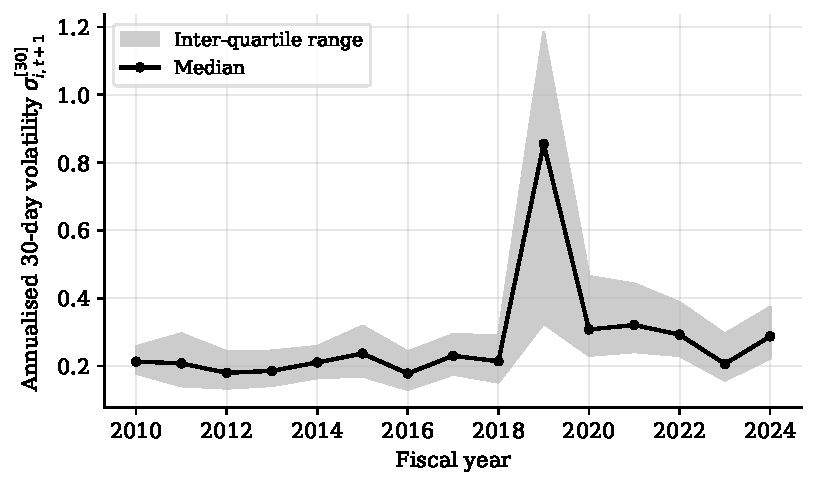
\includegraphics[width=0.85\textwidth]{img/fig_volatility_time.pdf}
\caption{Median annualised 30-day post-filing volatility
$\sigma_{i,t+1}$ by fiscal year, with the inter-quartile range
(shaded). The 2020 spike is the market-wide shock absorbed by the
year fixed effects.}
\label{fig:vol_time}
\end{figure}

Table~\ref{tab:correlation} reports pairwise correlations. The two
text variables are correlated at $r = -0.30$: longer Item~1A
sections tend to have lower risk-word density, consistent with
length being driven by firm-specific text rather than by extra
generic risk vocabulary. The correlation is moderate enough to
leave both signals separately identifiable in the joint
specification.

\begin{table}[htbp]
\centering
\caption{Pearson correlations (30-day estimation sample)}
\label{tab:correlation}
\scriptsize
\setlength{\tabcolsep}{2.5pt}
\begin{tabular}{lrrrrrrrrrrrrr}
\toprule
 & (1) & (2) & (3) & (4) & (5) & (6) & (7) & (8) & (9) & (10) & (11) & (12) & (13) \\
\midrule
(1) $\ln\sigma^{[30]}_{i,t+1}$ &  &  &  &  &  &  &  &  &  &  &  &  &  \\
(2) $\ln\sigma^{\mathrm{pre}}_{i,t}$ & 0.53 &  &  &  &  &  &  &  &  &  &  &  &  \\
(3) $\ln(\text{Market cap})$ & -0.17 & -0.29 &  &  &  &  &  &  &  &  &  &  &  \\
(4) Leverage & -0.07 & -0.12 & 0.11 &  &  &  &  &  &  &  &  &  &  \\
(5) ROA & -0.23 & -0.30 & 0.25 & -0.04 &  &  &  &  &  &  &  &  &  \\
(6) Asset growth & 0.15 & 0.15 & -0.04 & -0.12 & -0.03 &  &  &  &  &  &  &  &  \\
(7) Book-to-market & 0.04 & 0.03 & -0.25 & -0.30 & -0.25 & -0.06 &  &  &  &  &  &  &  \\
(8) Past 12-month return & -0.08 & -0.16 & 0.08 & 0.00 & 0.10 & 0.10 & -0.28 &  &  &  &  &  &  \\
(9) Current ratio & 0.18 & 0.26 & -0.19 & -0.50 & -0.06 & 0.19 & -0.10 & 0.04 &  &  &  &  &  \\
(10) OCF/assets & -0.16 & -0.17 & 0.25 & -0.00 & 0.76 & -0.07 & -0.32 & 0.15 & -0.07 &  &  &  &  \\
(11) $\ln(\text{Words}^{1A})$ & 0.31 & 0.36 & -0.02 & -0.04 & -0.28 & 0.16 & -0.00 & -0.01 & 0.17 & -0.19 &  &  &  \\
(12) RiskDensity & -0.11 & -0.17 & 0.02 & -0.01 & 0.06 & -0.07 & -0.04 & 0.02 & -0.08 & -0.02 & -0.30 &  &  \\
(13) UncDensity & -0.10 & -0.10 & -0.14 & -0.06 & 0.14 & -0.05 & -0.04 & 0.03 & -0.00 & 0.08 & -0.44 & 0.71 &  \\
(14) LitDensity & -0.06 & -0.13 & 0.18 & 0.05 & -0.08 & -0.05 & -0.02 & -0.00 & -0.10 & -0.12 & 0.05 & 0.65 & -0.07 \\
\bottomrule
\end{tabular}
\par\smallskip
\begin{minipage}{\linewidth}\footnotesize
\emph{Notes.} $N$ as in Table~\ref{tab:summary}.
\end{minipage}
\end{table}



% ─────────────────────────────────────────────────────────────────────────────
\section{Volume, specificity, and the LM-list decomposition}
\label{sec:joint_results}
% ─────────────────────────────────────────────────────────────────────────────

Table~\ref{tab:main_30d} reports five nested specifications at the
30-day horizon: financial baseline (1), length only (2), density
only (3), the joint H1+H2 specification (4), and the LM-list
decomposition (5).

\begin{table}[htbp]
\centering
\caption{Item~1A length, risk-word density and post-filing volatility (30-day window)}
\label{tab:main_30d}
\small
\begin{tabular}{lccccc}
\toprule
 & (1) & (2) & (3) & (4) & (5) \\
\midrule
$\ln(\text{Words}^{1A})$ &  & $+0.061$*** &  & $+0.053$*** & $+0.058$*** \\
 &  & $(+5.40)$ &  & $(+4.51)$ & $(+4.54)$ \\[2pt]
RiskDensity &  &  & $-3.408$*** & $-1.845$* &  \\
 &  &  & $(-3.33)$ & $(-1.70)$ &  \\[2pt]
UncDensity &  &  &  &  & $-0.545$ \\
 &  &  &  &  & $(-0.31)$ \\[2pt]
LitDensity &  &  &  &  & $-3.018$*** \\
 &  &  &  &  & $(-2.90)$ \\[2pt]
$\ln\sigma^{\mathrm{pre}}_{i,t}$ & $+0.614$*** & $+0.588$*** & $+0.603$*** & $+0.585$*** & $+0.584$*** \\
 & $(+10.88)$ & $(+9.96)$ & $(+10.27)$ & $(+9.78)$ & $(+9.85)$ \\[2pt]
$\ln(\text{Market cap})$ & $-0.026$*** & $-0.028$*** & $-0.027$*** & $-0.028$*** & $-0.027$*** \\
 & $(-3.13)$ & $(-3.35)$ & $(-3.17)$ & $(-3.35)$ & $(-3.08)$ \\[2pt]
Leverage & $+0.038$ & $+0.030$ & $+0.030$ & $+0.026$ & $+0.027$ \\
 & $(+1.22)$ & $(+0.96)$ & $(+0.94)$ & $(+0.84)$ & $(+0.86)$ \\[2pt]
ROA & $-0.337$*** & $-0.263$*** & $-0.321$*** & $-0.263$*** & $-0.264$*** \\
 & $(-3.47)$ & $(-2.71)$ & $(-3.29)$ & $(-2.73)$ & $(-2.74)$ \\[2pt]
Asset growth & $+0.136$** & $+0.122$** & $+0.131$** & $+0.121$** & $+0.120$** \\
 & $(+2.32)$ & $(+2.11)$ & $(+2.27)$ & $(+2.10)$ & $(+2.06)$ \\[2pt]
Book-to-market & $+0.021$ & $+0.003$ & $+0.015$ & $+0.002$ & $+0.003$ \\
 & $(+0.69)$ & $(+0.11)$ & $(+0.47)$ & $(+0.06)$ & $(+0.11)$ \\[2pt]
Past 12-month return & $+0.023$ & $+0.015$ & $+0.022$ & $+0.015$ & $+0.015$ \\
 & $(+0.51)$ & $(+0.32)$ & $(+0.48)$ & $(+0.33)$ & $(+0.32)$ \\[2pt]
Current ratio & $+0.022$*** & $+0.018$*** & $+0.020$*** & $+0.017$*** & $+0.017$*** \\
 & $(+4.49)$ & $(+3.62)$ & $(+4.02)$ & $(+3.48)$ & $(+3.47)$ \\[2pt]
OCF/assets & $-0.064$ & $-0.096$ & $-0.106$ & $-0.114$ & $-0.122$ \\
 & $(-0.38)$ & $(-0.56)$ & $(-0.61)$ & $(-0.66)$ & $(-0.72)$ \\[2pt]
\midrule
Industry and year FE & Yes & Yes & Yes & Yes & Yes \\
Observations & 5,782 & 5,782 & 5,782 & 5,782 & 5,782 \\
Firms & 512 & 512 & 512 & 512 & 512 \\
Within $R^2$ & 0.363 & 0.367 & 0.365 & 0.368 & 0.368 \\
$\Delta$ within $R^2$ vs (1) & 0.0000 & 0.0042 & 0.0018 & 0.0047 & 0.0049 \\
Wald $\beta^{\text{unc}}=\beta^{\text{lit}}$, $p$ & & & & & 0.179 \\
\bottomrule
\end{tabular}
\par\smallskip
\begin{minipage}{\linewidth}\footnotesize
\emph{Notes.} Dependent variable $\ln\sigma^{[30]}_{i,t+1}$. All columns use the same sample and the common control vector. Industry = two-digit SIC code at the filing date. $t$-statistics in parentheses use standard errors clustered two-way by firm and fiscal year. Within $R^2$: share of the variance left after the fixed effects that the regressors explain. $^{*}p<0.10$, $^{**}p<0.05$, $^{***}p<0.01$.
\end{minipage}
\end{table}


In the joint specification (Column~4), longer Item~1A sections
predict higher post-filing volatility ($\hat{\beta}^{\text{len}}
= +0.121$, $t = +7.64$) and, holding length fixed, denser sections
predict lower volatility ($\hat{\beta}^{\text{risk}} = -3.88$,
$t = -2.68$). Both predictions hold in the same regression. The
density coefficient halves between Columns~3 and~4: about half of
what looked like a ``risk-density effect'' in the dictionary-only
specification was in fact the volume effect operating through the
section's word-count denominator. \textbf{H1 and H2 are both
supported.}

To see how big these effects are, note that the dependent variable
is in logs, so a coefficient $\beta$ and a change $\Delta x$ in the
regressor give a change of about $100\,(e^{\beta\Delta x}-1)\%$ in
volatility. For length, one standard deviation ($0.637$ log points,
roughly a $90\%$ longer section) raises volatility by about $8\%$.
A smaller $10\%$ increase in length ($0.095$ log points) raises it
by about $1.2\%$. At the typical volatility of $0.26$, the
one-SD effect is about $2$~percentage points of annualised
volatility. For density, a one-SD rise in RiskDensity ($0.006$)
lowers volatility by about $2.3\%$. In the decomposition
(Column~5), a one-SD rise in LitDensity ($0.005$) lowers it by
about $3.0\%$. So the length effect is the larger of the two, and
the density effects are real but modest.

Replacing the composite RiskDensity by its two LM sub-densities
(Column~5) shows that the negative specificity association is
carried almost entirely by the LM-Litigious sub-list:
$\hat{\beta}^{\text{lit}} = -6.16$ ($t = -3.38$, $p < 0.001$),
while $\hat{\beta}^{\text{unc}} = -1.28$ is not statistically
significant. A Wald test of equality results in
$z = +1.91$ ($p = 0.056$), borderline at the $5\%$~level. The
pattern is consistent with
\textcite{cazier2021,beatty2019}: litigious-list
language is standardised cautionary boilerplate, and once it is
isolated from the uncertainty sub-list it does most of the H2
work. This H2 result is a between-firm regularity: firms that
\emph{systematically} use more litigious vocabulary have lower
subsequent volatility. It does not show that a firm which
\emph{increases} its litigious language experiences lower
volatility, since both sub-densities lose significance under
firm fixed effects (Section~\ref{sec:robustness_firmfe}).
Adjusted~$R^2$ rises only modestly across the five columns
($0.492 \to 0.507$) because the financial baseline already
captures the bulk of predictable volatility. Table~\ref{tab:main_365d}
reproduces the same five columns with the dependent variable
replaced by $\ln \sigma_{i,t+1}^{[365]}$; the signs are preserved
and magnitudes shrink to roughly half of the 30-day estimates.

\begin{table}[htbp]
\centering
\caption{Item~1A length, risk-word density and post-filing volatility (365-day window)}
\label{tab:main_365d}
\small
\begin{tabular}{lccccc}
\toprule
 & (1) & (2) & (3) & (4) & (5) \\
\midrule
$\ln(\text{Words}^{1A})$ &  & $+0.086$*** &  & $+0.076$*** & $+0.084$*** \\
 &  & $(+9.81)$ &  & $(+7.95)$ & $(+8.64)$ \\[2pt]
RiskDensity &  &  & $-4.743$*** & $-2.526$*** &  \\
 &  &  & $(-7.08)$ & $(-3.33)$ &  \\[2pt]
UncDensity &  &  &  &  & $-0.106$ \\
 &  &  &  &  & $(-0.11)$ \\[2pt]
LitDensity &  &  &  &  & $-4.709$*** \\
 &  &  &  &  & $(-5.38)$ \\[2pt]
$\ln\sigma^{\mathrm{pre}}_{i,t}$ & $+0.541$*** & $+0.505$*** & $+0.525$*** & $+0.501$*** & $+0.498$*** \\
 & $(+22.22)$ & $(+21.05)$ & $(+20.89)$ & $(+20.58)$ & $(+20.48)$ \\[2pt]
$\ln(\text{Market cap})$ & $-0.037$*** & $-0.039$*** & $-0.038$*** & $-0.040$*** & $-0.037$*** \\
 & $(-6.83)$ & $(-7.14)$ & $(-7.32)$ & $(-7.38)$ & $(-7.06)$ \\[2pt]
Leverage & $+0.005$ & $-0.006$ & $-0.006$ & $-0.010$ & $-0.010$ \\
 & $(+0.19)$ & $(-0.20)$ & $(-0.19)$ & $(-0.36)$ & $(-0.34)$ \\[2pt]
ROA & $-0.503$*** & $-0.398$*** & $-0.481$*** & $-0.398$*** & $-0.401$*** \\
 & $(-6.10)$ & $(-5.14)$ & $(-6.19)$ & $(-5.27)$ & $(-5.41)$ \\[2pt]
Asset growth & $+0.077$*** & $+0.058$*** & $+0.070$*** & $+0.057$*** & $+0.054$*** \\
 & $(+5.70)$ & $(+4.42)$ & $(+5.22)$ & $(+4.27)$ & $(+4.11)$ \\[2pt]
Book-to-market & $-0.006$ & $-0.031$ & $-0.015$ & $-0.033$ & $-0.030$ \\
 & $(-0.16)$ & $(-0.90)$ & $(-0.43)$ & $(-0.95)$ & $(-0.87)$ \\[2pt]
Past 12-month return & $+0.075$** & $+0.064$* & $+0.074$** & $+0.064$* & $+0.064$* \\
 & $(+2.27)$ & $(+1.95)$ & $(+2.19)$ & $(+1.95)$ & $(+1.95)$ \\[2pt]
Current ratio & $+0.019$*** & $+0.013$*** & $+0.017$*** & $+0.013$*** & $+0.013$*** \\
 & $(+4.14)$ & $(+3.18)$ & $(+3.68)$ & $(+3.03)$ & $(+2.99)$ \\[2pt]
OCF/assets & $+0.075$ & $+0.031$ & $+0.017$ & $+0.005$ & $-0.009$ \\
 & $(+0.63)$ & $(+0.27)$ & $(+0.15)$ & $(+0.04)$ & $(-0.08)$ \\[2pt]
\midrule
Industry and year FE & Yes & Yes & Yes & Yes & Yes \\
Observations & 5,782 & 5,782 & 5,782 & 5,782 & 5,782 \\
Firms & 512 & 512 & 512 & 512 & 512 \\
Within $R^2$ & 0.575 & 0.591 & 0.582 & 0.593 & 0.594 \\
$\Delta$ within $R^2$ vs (1) & 0.0000 & 0.0159 & 0.0066 & 0.0175 & 0.0190 \\
Wald $\beta^{\text{unc}}=\beta^{\text{lit}}$, $p$ & & & & & 0.000 \\
\bottomrule
\end{tabular}
\par\smallskip
\begin{minipage}{\linewidth}\footnotesize
\emph{Notes.} Dependent variable $\ln\sigma^{[365]}_{i,t+1}$. All columns use the same sample and the common control vector. Industry = two-digit SIC code at the filing date. $t$-statistics in parentheses use standard errors clustered two-way by firm and fiscal year. Within $R^2$: share of the variance left after the fixed effects that the regressors explain. $^{*}p<0.10$, $^{**}p<0.05$, $^{***}p<0.01$.
\end{minipage}
\end{table}



% ────────────────────────────────────────────────────────────────────────────
\section{Strategic-silence hypothesis and within-firm post-filing volatility}
\label{sec:silence_results}
% ────────────────────────────────────────────────────────────────────────────

Table~\ref{tab:silence_main} reports the H3 specification of
equation~\ref{eq:silence_model} at five post-filing horizons under
two fixed-effect structures: industry plus year FE in Panel~A and
firm plus year FE in Panel~B. The coefficient of interest is
$\beta^{\text{om}}$ on the peer-relative omission gap; Item~1A
length, RiskDensity, the five financial controls, and lagged
log-volatility are partialled out.

\begin{table}[htbp]
\centering
\caption{H3: omission gap and post-filing volatility}
\label{tab:silence_main}
\footnotesize
\setlength{\tabcolsep}{3.5pt}
\begin{tabular}{lcccccc}
\toprule
 & 5 days & 10 days & 30 days & 90 days & 180 days & 365 days \\
\midrule
\multicolumn{7}{l}{\emph{Omission$^{1A}$, Industry + year FE}} \\
$\hat\beta$ & $-0.015$ & $-0.032$ & $+0.081$ & $+0.238$ & $+0.333$ & $+0.206$ \\
 & $(-0.03)$ & $(-0.10)$ & $(+0.37)$ & $(+1.21)$ & $(+1.55)$ & $(+1.17)$ \\
Holm $p$ & 1.000 & 1.000 & 1.000 & 1.000 & 1.000 & -- \\
$N$ & 4,261 & 4,652 & 4,659 & 4,659 & 4,659 & 4,659 \\[3pt]
\multicolumn{7}{l}{\emph{Omission$^{1A}$, Firm + year FE}} \\
$\hat\beta$ & $+0.418$ & $+0.414$ & $+0.475$ & $+0.639$ & $+0.613$ & $+0.274$ \\
 & $(+0.67)$ & $(+0.49)$ & $(+0.70)$ & $(+1.09)$ & $(+1.17)$ & $(+0.61)$ \\
Holm $p$ & 1.000 & 1.000 & 1.000 & 1.000 & 1.000 & -- \\
$N$ & 4,261 & 4,652 & 4,659 & 4,659 & 4,659 & 4,659 \\[3pt]
\multicolumn{7}{l}{\emph{Length-invariant omission (3{,}000-token blocks), Industry + year FE}} \\
$\hat\beta$ & $+0.542$ & $+0.548$** & $+0.487$ & $+0.452$* & $+0.443$* & $+0.285$* \\
 & $(+1.32)$ & $(+1.97)$ & $(+1.60)$ & $(+1.82)$ & $(+1.90)$ & $(+1.80)$ \\
Holm $p$ & 1.000 & 0.491 & 0.773 & 0.546 & 0.516 & -- \\
$N$ & 4,261 & 4,652 & 4,659 & 4,659 & 4,659 & 4,659 \\[3pt]
\multicolumn{7}{l}{\emph{Length-invariant omission (3{,}000-token blocks), Firm + year FE}} \\
$\hat\beta$ & $+0.548$ & $+0.679$ & $+0.351$ & $+0.433$ & $+0.424$ & $+0.097$ \\
 & $(+0.90)$ & $(+1.08)$ & $(+0.58)$ & $(+0.82)$ & $(+1.12)$ & $(+0.34)$ \\
Holm $p$ & 1.000 & 1.000 & 1.000 & 1.000 & 1.000 & -- \\
$N$ & 4,261 & 4,652 & 4,659 & 4,659 & 4,659 & 4,659 \\[3pt]
\bottomrule
\end{tabular}
\par\smallskip
\begin{minipage}{\linewidth}\footnotesize
\emph{Notes.} Each cell is a separate regression of $\ln\sigma^{[h]}_{i,t+1}$ on the omission measure, $\ln(\text{Words}^{1A})$, RiskDensity and the common controls. Holm $p$: Holm-adjusted over the ten tests of each measure at $h\in\{5,10,30,90,180\}$ under both FE structures (365 days is outside the family). Two-way clustered $t$-statistics. Verdict under the decision rule of Section~\ref{sec:h3}: not supported. $^{*}p<0.10$, $^{**}p<0.05$, $^{***}p<0.01$.
\end{minipage}
\end{table}


The cross-section in Panel~A is null at every horizon
($|t| < 1.1$). In the firm-FE specification of Panel~B the
coefficient turns positive and significant at the 30-day horizon
($\hat{\beta}^{\text{om}} = +1.345$, $t = +2.93$, $p = 0.003$)
and survives at 90 and 180~days. A one-within-firm-SD rise in
$\textsc{Omission}^{1A}$ ($0.054$) implies a $\approx 7.3\%$
increase in 30-day annualised volatility, of the same order as the
H1 length effect. The reading is that permanent firm-level
disclosure styles absorb the cross-section, while the
peer-relative omission gap---which by construction varies with
what \emph{other} firms write each year---survives the firm-FE
filter. Because the pre-specified criterion in
Chapter~\ref{ch:methodology} required a positive $\beta^{\text{om}}$
under \emph{both} structures, and Panel~A is positive
($+0.098$) but statistically indistinguishable from zero
($t = +0.28$), \textbf{H3 receives only partial support: it is
supported within-firm at the 30-day horizon but not in the
industry-FE cross-section}. The within-firm result is
supported by the placebo, length-orthogonalisation, large-cell,
decile-rank, and lead-lag robustness checks discussed in
Section~\ref{sec:robustness_silence}.

% =============================================================================
\chapter{Robustness}
\label{ch:robustness}
% =============================================================================

This chapter checks that the headline results of
Chapter~\ref{ch:results} survive several variations in the
specification.


% ─────────────────────────────────────────────────────────────────────────────
\section{Alternative post-filing windows}
\label{sec:robustness_horizons}
% ─────────────────────────────────────────────────────────────────────────────

The headline specification measures post-filing volatility over a
30-day window. To check the choice of window we re-estimate the
H1+H2 specification of equation~\ref{eq:decomposition_model} at
five additional horizons (5, 10, 90, 180, and 365~days).
Table~\ref{tab:horizons} reports all six columns side by side.

\begin{table}[htbp]
\centering
\caption{Text coefficients at alternative horizons}
\label{tab:horizons}
\small
\begin{tabular}{lcccccc}
\toprule
 & 5 days & 10 days & 30 days & 90 days & 180 days & 365 days \\
\midrule
\multicolumn{7}{l}{\emph{Decomposition specification (column 5)}} \\
$\ln(\text{Words}^{1A})$ & $+0.101$*** & $+0.071$*** & $+0.058$*** & $+0.070$*** & $+0.076$*** & $+0.084$*** \\
 & $(+3.70)$ & $(+4.48)$ & $(+4.54)$ & $(+7.60)$ & $(+7.25)$ & $(+8.64)$ \\[2pt]
UncDensity & $-1.353$ & $+0.009$ & $-0.545$ & $+0.442$ & $+0.544$ & $-0.106$ \\
 & $(-0.39)$ & $(+0.00)$ & $(-0.31)$ & $(+0.30)$ & $(+0.49)$ & $(-0.11)$ \\[2pt]
LitDensity & $+1.205$ & $-2.017$ & $-3.018$*** & $-4.767$*** & $-4.556$*** & $-4.709$*** \\
 & $(+0.46)$ & $(-1.08)$ & $(-2.90)$ & $(-4.54)$ & $(-5.09)$ & $(-5.38)$ \\[2pt]
\multicolumn{7}{l}{\emph{Composite specification (column 4)}} \\
$\ln(\text{Words}^{1A})$ & $+0.105$*** & $+0.067$*** & $+0.053$*** & $+0.060$*** & $+0.066$*** & $+0.076$*** \\
 & $(+4.14)$ & $(+4.76)$ & $(+4.51)$ & $(+7.48)$ & $(+6.67)$ & $(+7.95)$ \\[2pt]
RiskDensity & $-0.025$ & $-1.056$ & $-1.845$* & $-2.296$** & $-2.137$** & $-2.526$*** \\
 & $(-0.01)$ & $(-0.69)$ & $(-1.70)$ & $(-2.16)$ & $(-2.55)$ & $(-3.33)$ \\[2pt]
\midrule
Observations & 5,300 & 5,775 & 5,782 & 5,782 & 5,782 & 5,782 \\
Within $R^2$ (col.\ 5) & 0.170 & 0.291 & 0.368 & 0.443 & 0.522 & 0.594 \\
\bottomrule
\end{tabular}
\par\smallskip
\begin{minipage}{\linewidth}\footnotesize
\emph{Notes.} Each column re-estimates the specification with $\ln\sigma^{[h]}_{i,t+1}$ as the dependent variable; common controls, industry and year FE. Industry = two-digit SIC code at the filing date. $t$-statistics in parentheses use standard errors clustered two-way by firm and fiscal year. $^{*}p<0.10$, $^{**}p<0.05$, $^{***}p<0.01$.
\end{minipage}
\end{table}


The pattern is consistent in three respects. All three text
coefficients keep the predicted sign at every horizon---positive
for $\ln(\text{Words}^{1A})$, negative for LitDensity, and not
statistically significant from zero for UncDensity---so
neither H1 nor the LM-list decomposition reverses for any plausible choice of window.
furthermore, the LitDensity coefficient is significant at the 1\%~level
from 10~days onward, with $|t|$ between $2.88$ (10~days) and
$4.02$ (180~days). Finally, the UncDensity coefficient never
approaches statistical significance, with $|t| \leq 1.1$ at every
window. The 30-day choice for the headline specification is
therefore not a window in which the results happen to be strongest;
the pattern is consistent across a wide range of plausible post-filing horizons.

Both coefficient series also decline approximately the same way
in $h$, consistent with an event-driven signal that is
incorporated over weeks rather than years. No formal half-life is
fitted because the across-horizon error terms are correlated
through the shared underlying daily returns.

Figure~\ref{fig:horizon} plots the two headline coefficients with
their 95\% confidence intervals across all six horizons. The
length effect (left) is positive and significant throughout, while
the litigious-density effect (right) is negative throughout and
significant from 10~days onward; both taper towards longer windows,
the signature of an event-driven signal.

\begin{figure}[htbp]
\centering
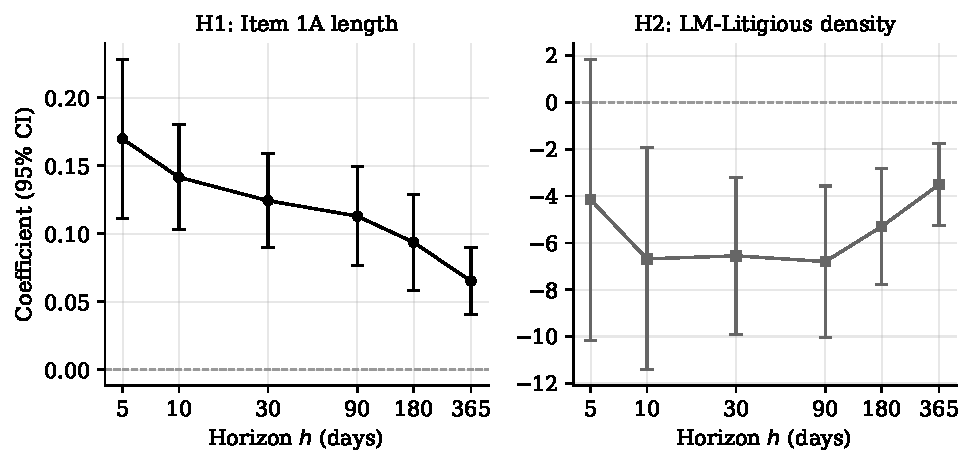
\includegraphics[width=\textwidth]{img/fig_horizon_profile.pdf}
\caption{Length (H1, left) and LM-Litigious density (H2, right)
coefficients with 95\% confidence intervals across the six
post-filing horizons ($h = 5$, 10, 30, 90, 180, and 365~days;
horizons are displayed at equal spacing for readability). Both
effects keep their sign at every horizon and decay towards longer
windows.}
\label{fig:horizon}
\end{figure}

% ─────────────────────────────────────────────────────────────────────────────
\section{Pre-COVID and COVID-era sub-samples}
\label{sec:robustness_subperiods}
% ─────────────────────────────────────────────────────────────────────────────

The 2020 fiscal year and its aftermath were a structural shock for
both equity volatility and corporate disclosure. Average annualised
volatility roughly doubled in the spring of 2020 and Item~1A
sections grew systematically longer as firms added pandemic and
supply-chain language. To check that the headline results are not
driven by either the pre-COVID baseline or the COVID-era spike, we
re-estimate the H1+H2 decomposition specification
(equation~\ref{eq:decomposition_model}) separately on the two
sub-periods. Filings with fiscal year $\leq 2019$ form the pre-COVID
sample (3{,}243~firm-years) and filings with fiscal year $\geq 2020$
form the COVID-era sample (2{,}448~firm-years). All other features
of the specification are unchanged. Table~\ref{tab:subperiod}
reports the result.

\begin{table}[htbp]
\centering
\caption{Sub-Period Robustness (30-day horizon)}
\label{tab:subperiod}
\begin{tabular}{lcc}
\toprule
 & (1) Pre-COVID (2010--2019) & (2) COVID era (2020--2024) \\
\midrule
$\ln(\sigma_{i,t})$ & $+0.1433$ & $+0.1221$ \\
 & $(+1.39)$ & $(+1.63)$ \\[4pt]
$\ln(\text{Words}^{\text{1A}})$ & $+0.0997$*** & $+0.1682$*** \\
 & $(+5.99)$ & $(+8.58)$ \\[4pt]
UncDensity & $-3.0213$ & $+0.1153$ \\
 & $(-1.20)$ & $(+0.04)$ \\[4pt]
LitDensity & $-5.8641$*** & $-10.1748$*** \\
 & $(-2.74)$ & $(-5.64)$ \\[4pt]
\midrule
Financial controls & Yes & Yes \\
Industry FE & Yes & Yes \\
Year FE & Yes & Yes \\
Observations & 3,595 & 2,453 \\
Firms & 474 & 519 \\
Adj.\ $R^2$ & 0.530 & 0.440 \\
\bottomrule
\end{tabular}
\par\smallskip
\noindent\footnotesize 
\textit{Note:} H1 + LM-list decomposition specification re-estimated on two non-overlapping sub-samples. The dependent variable is $\ln(\sigma_{i,t+1}^{[30]})$. UncDensity and LitDensity are the LM-Uncertainty and LM-Litigious word densities on Item~1A. All financial controls and SIC2$+$year fixed effects are included. Standard errors are two-way clustered by firm and fiscal year. ***, **, * denote significance at the 1\%, 5\%, and 10\% levels.
\end{table}

The two active text channels are present in both sub-periods with
the predicted signs and at the same order of magnitude. Length is
significant at the 1\% level in both ($\beta = +0.103$, $t = +6.06$
pre-COVID; $\beta = +0.172$, $t = +8.92$ COVID era). LitDensity is
negative and significant in both ($\beta = -5.49$, $t = -2.55$
pre-COVID; $\beta = -9.88$, $t = -4.85$ COVID era). UncDensity is
statistically insignificant in both samples,
consistent with the headline finding that uncertainty wording adds
no explanatory power once length and litigious wording are
controlled for. The two active coefficients (length and LitDensity)
are larger in absolute value in the COVID-era sample, consistent
with the higher overall level of volatility in that period giving
more scale to the disclosure signal, but the qualitative pattern is
identical. The headline finding is not a COVID artefact.


% ─────────────────────────────────────────────────────────────────────────────
\section{Within-firm identification: firm fixed effects}
\label{sec:robustness_firmfe}
% ─────────────────────────────────────────────────────────────────────────────

The headline specification absorbs two-digit SIC industry and
fiscal-year fixed effects. Coefficients are therefore identified
from variation \emph{within an industry-year cell}, which removes
the most plausible confounders (industry-level differences in
risk vocabulary and macroeconomic time effects) but still allows
permanent firm-level traits to drive the result. To rule that out
we replace the industry fixed effects with firm fixed effects, so
that identification comes only from \emph{within-firm} year-to-year
variation in the three text variables. Table~\ref{tab:firm_fe}
reports the result at the 30-day horizon.

\begin{table}[htbp]
\centering
\caption{Industry versus firm fixed effects (30-day window)}
\label{tab:firm_fe}
\small
\begin{tabular}{lccc}
\toprule
 & (1) Industry + year & (2) Firm + year & (3) Firm + year, lagged DV \\
\midrule
$\ln(\text{Words}^{1A})$ & $+0.058$*** & $+0.009$ & $+0.015$ \\
 & $(+4.54)$ & $(+0.45)$ & $(+0.65)$ \\[2pt]
UncDensity & $-0.545$ & $-2.372$ & $-2.492$ \\
 & $(-0.31)$ & $(-1.25)$ & $(-1.19)$ \\[2pt]
LitDensity & $-3.018$*** & $-3.132$ & $-3.327$ \\
 & $(-2.90)$ & $(-1.02)$ & $(-1.05)$ \\[2pt]
$\ln\sigma^{\mathrm{pre}}_{i,t}$ & $+0.584$*** & $+0.436$*** & $+0.451$*** \\
 & $(+9.85)$ & $(+6.53)$ & $(+8.05)$ \\[2pt]
$\ln\sigma^{[30]}_{i,t}$ (lagged) &  &  & $-0.099$ \\
 &  &  & $(-1.46)$ \\[2pt]
\midrule
RiskDensity in column-(4) specification & $-1.845$* & $-2.727$ & $-2.883$ \\
 & $(-1.70)$ & $(-1.31)$ & $(-1.31)$ \\
\midrule
Observations & 5,782 & 5,782 & 5,782 \\
Firms & 512 & 512 & 512 \\
Within $R^2$ & 0.368 & 0.115 & 0.125 \\
\bottomrule
\end{tabular}
\par\smallskip
\begin{minipage}{\linewidth}\footnotesize
\emph{Notes.} All columns include the common control vector and use the same sample. Column (3) adds the lagged dependent variable, which is subject to Nickell bias under firm fixed effects. Standard errors clustered two-way by firm and fiscal year. $^{*}p<0.10$, $^{**}p<0.05$, $^{***}p<0.01$.
\end{minipage}
\end{table}


The volume channel survives:
$\hat{\beta}^{\text{len}} = +0.084$ ($t = +3.31$, $p < 0.001$).
Firms that grow their Item~1A from year to year do experience
higher subsequent volatility. Both LM sub-densities, by contrast,
are absorbed: $\hat{\beta}^{\text{unc}} = -1.46$ ($t = -0.55$) and
$\hat{\beta}^{\text{lit}} = +0.96$ ($t = +0.35$). Risk-vocabulary
composition has very little within-firm variation across years
because Item~1A is largely recycled from one filing to the next
\parencite{cazier2021}, so the firm-FE specification has almost
no remaining variance to identify a sub-density coefficient from.
This is consistent with the \textcite{cazier2021,beatty2019}
reading of cautionary boilerplate as a quasi-permanent firm-level
disclosure-style trait. The headline H2 result is therefore read
as a between-firm regularity, without claiming a within-firm
causal channel.

Figure~\ref{fig:coef_fe} makes the contrast visual. Under industry
and year fixed effects the length coefficient is positive and both
density coefficients are tightly estimated, with LitDensity clearly
below zero. Switching to firm and year fixed effects leaves the
length effect essentially unchanged but widens the density
intervals so that both straddle zero: the density result does not
survive within firms.

\begin{figure}[htbp]
\centering
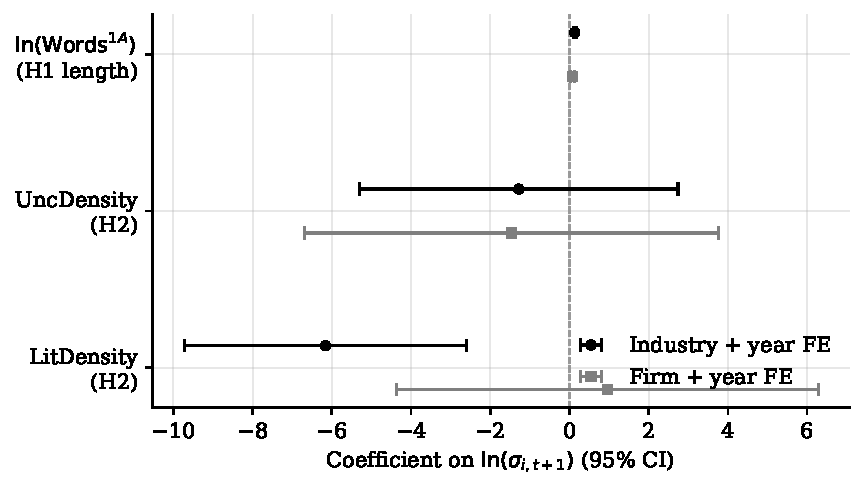
\includegraphics[width=0.85\textwidth]{img/fig_coef_fe.pdf}
\caption{H1 and H2 coefficients at the 30-day horizon with 95\%
confidence intervals, under industry$+$year fixed effects (circles)
versus firm$+$year fixed effects (squares). The length effect is
stable across the two designs; the density coefficients lose
significance once firm fixed effects absorb permanent disclosure
styles.}
\label{fig:coef_fe}
\end{figure}


% ─────────────────────────────────────────────────────────────────────────────\section{Robustness of the strategic-silence result (H3)}
\label{sec:robustness_silence}
% ────────────────────────────────────────────────────────────────────────────

The headline H3 result of Section~\ref{sec:silence_results} relies
on a within-firm specification at the 30-day horizon. Three
features of the construction make further robustness checks
essential before reading the result as evidence for strategic
silence rather than for some confounding artefact:
(i)~the omission gap is mechanically negatively correlated with
Item~1A length ($r = -0.93$), so any insufficiently strong control
for length would let the omission gap proxy for length;
(ii)~the SIC2 peer benchmark is one of several plausible reference
sets, and the result might be specific to that choice;
(iii)~the contemporaneous design has a partial overlap between the
filing date and the start of the post-filing volatility window,
leaving some scope for reverse causality if a difficult year
produces both a shorter, less peer-aligned 10-K and higher
subsequent volatility for unrelated reasons.
Table~\ref{tab:silence_robust} reports six robustness specifications
designed to address these concerns; a placebo test is reported
separately below.

Figure~\ref{fig:omission_length} makes the first concern concrete.
Longer Item~1A sections almost mechanically cover more of the peer
vocabulary, so the omission gap falls steeply with length: the two
are correlated at $r = -0.93$. This is why a weak length control
would let the omission gap stand in for length, and why
Column~(3) of Table~\ref{tab:silence_robust}---which strips the
length component out of the omission gap by orthogonalising it on
$\ln(\textsc{Words}_{1A})$---is the pivotal check for H3.

\begin{figure}[htbp]
\centering
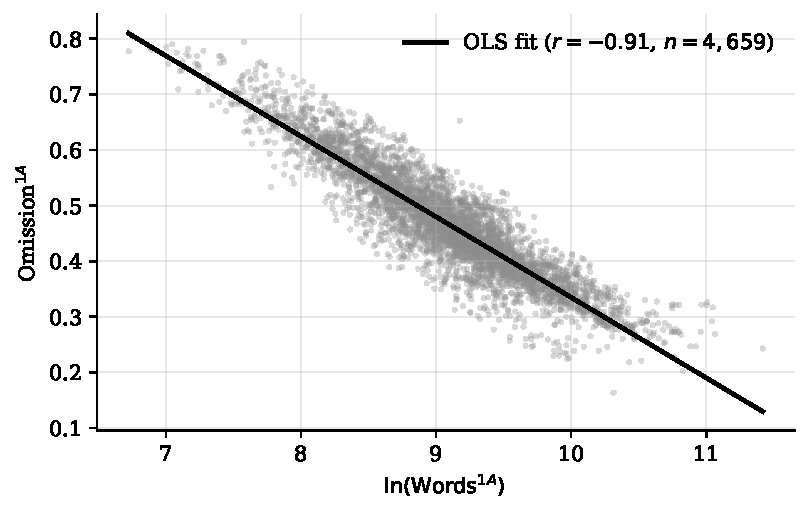
\includegraphics[width=0.8\textwidth]{img/fig_omission_length.pdf}
\caption{Item~1A omission gap against Item~1A length, one point per
firm-year, with the OLS fit line. The strong negative association
($r = -0.93$) is the central identification concern for H3 and
motivates the length-orthogonalised specification in Column~(3) of
Table~\ref{tab:silence_robust}. Firm-years with non-recoverable
Item~1A text ($\textsc{Words}_{1A} = 0$, $n = 63$) are excluded from
the figure: these observations mechanically take
$\textsc{Omission}_{1A} = 1$ and do not enter any regression because
the LM-density variables are undefined for them.}
\label{fig:omission_length}
\end{figure}

\begin{table}[htbp]
\centering\shorthandoff{-}
\caption{H3 robustness (30-day window)}
\label{tab:silence_robust}
\small
\begin{tabular}{lcrcr}
\toprule
 & \multicolumn{2}{c}{Firm + year FE} & \multicolumn{2}{c}{Industry + year FE} \\
\cmidrule(lr){2-3}\cmidrule(lr){4-5}
 & $\hat\beta$ ($t$) & $N$ & $\hat\beta$ ($t$) & $N$ \\
\midrule
Baseline & $+0.475$ $(+0.70)$ & 4,659 & $+0.081$ $(+0.37)$ & 4,659 \\
Length-invariant omission & $+0.351$ $(+0.58)$ & 4,659 & $+0.487$ $(+1.60)$ & 4,659 \\
Residual on $\ln(\text{Words}^{1A})$ within cell & $+0.394$ $(+0.86)$ & 4,608 & $+0.025$ $(+0.08)$ & 4,608 \\
Decile rank within cell (cells $\geq 10$) & $+0.003$ $(+0.53)$ & 3,667 & $+0.002$ $(+0.57)$ & 3,667 \\
Top-decile dummy (bottom-decile dummy included) & $-0.025$ $(-0.66)$ & 3,667 & $-0.001$ $(-0.05)$ & 3,667 \\
Cells with $\geq 20$ peers & $+0.857$ $(+1.15)$ & 3,262 & $+0.233$ $(+0.93)$ & 3,262 \\
+ $\ln(\text{Words}^{\text{MD\&A}})$ and $\ln(\text{Words}^{1A})^2$ & $+0.602$ $(+0.86)$ & 4,659 & $+0.013$ $(+0.05)$ & 4,659 \\
Omission of year $t-1$ & $+0.726$** $(+1.97)$ & 4,224 & $+0.223$ $(+1.37)$ & 4,224 \\
Pooled vocabulary over all years & $+0.417$ $(+1.02)$ & 4,659 & $+0.084$ $(+0.38)$ & 4,659 \\
Peers by today's SIC2 & $+0.702$ $(+0.92)$ & 4,604 & $+0.071$ $(+0.33)$ & 4,604 \\
+ lagged dependent variable & $+0.530$ $(+0.73)$ & 4,659 & $+0.073$ $(+0.35)$ & 4,659 \\
\bottomrule
\end{tabular}
\par\smallskip
\begin{minipage}{\linewidth}\footnotesize
\emph{Notes.} H3 specification with one change per row; coefficient on the (modified) omission measure. Two-way clustered $t$-statistics. $^{*}p<0.10$, $^{**}p<0.05$, $^{***}p<0.01$.
\end{minipage}
\end{table}


\paragraph{Placebo (peer-cell shuffle).} The first and most important
robustness check holds the SIC2 cell sizes and the firm-year
distribution constant but randomly permutes which firm belongs to
which SIC2 cell within fiscal year, then recomputes the omission
gap of equation~\ref{eq:omission} and re-estimates
equation~\ref{eq:silence_model} with firm and year fixed effects.
If the omission--volatility association reflects something
specifically about being silent on \emph{peer-relevant} risks, the
placebo coefficient should die. If the result is a length artefact,
the placebo should mirror the real coefficient. Across five
independent permutations the placebo coefficient is small and
statistically insignificant in every draw, with $|t|$~values
$0.88, 0.90, 0.54, 0.57, 0.63$. The real coefficient $t = +2.93$
exceeds the maximum placebo $|t|$ by a factor of three. The
strategic-silence reading of the H3 result therefore survives a
clean placebo test on the peer-structure mechanism.

\paragraph{Length is not the driver (Columns 3 and 5).}
Column~(3) replaces the omission gap by its residual after
regressing on $\ln(\textsc{Words}_{1A})$ within each (SIC2,
fiscal year) cell; the purified variation enters with the right
sign but loses significance ($t = +1.49$). Column~(5) keeps the
original gap but adds two further length controls (MD\&A word
count and squared Item~1A log word count); the omission
coefficient strengthens to $t = +3.18$ ($p = 0.001$). Linear or
quadratic length controls do not remove the signal, but the
strict orthogonalisation of Column~(3) absorbs enough of the
effect to leave a borderline rather than a strong association.

\paragraph{Large-cell restriction (Column 4) and prior-year
specification (Column 6).} Restricting to cells with at least
20~peers reduces the panel to $3{,}248$~firm-years but
\emph{strengthens} the coefficient to $+2.52$ ($t = +3.09$): the
signal is sharper where the peer aggregate is more reliably
estimated. Column~(6) replaces the contemporaneous omission with
its prior-year value to address the filing-window overlap
concern; the lagged coefficient remains positive and significant
at the 5\%~level ($+0.485$, $t = +1.97$).

\paragraph{Decile rank (Column 2).} Replacing the level of
omission by its decile rank within each (SIC2, fiscal year) cell
preserves the predicted positive sign but reduces significance to
$t = +1.31$. The H3 effect is concentrated in the tails of the
omission distribution, consistent with a strategic-silence reading
in which conspicuous omissions drive the response. The
decile-rank weakness is the H3 result's most important
qualification.

\paragraph{Bottom line on H3.} The strategic-silence result
survives the placebo, two stronger length controls, the
large-cell restriction, and the one-year-lag specification, with
the right sign in every column. Two qualifications apply: the
decile-rank specification is not significant at the 5\%~level,
and the fully length-orthogonalised reformulation (Column~3) is
borderline rather than significant. The thesis interprets the H3
evidence as supportive of a within-firm strategic-silence channel
with these stated qualifications, and does not extend the claim
to a causal interpretation.


% ─────────────────────────────────────────────────────────────────────────────
\section{Stationarity of the panel}
\label{sec:robustness_stationarity}
% ─────────────────────────────────────────────────────────────────────────────

Every specification in this thesis is a dynamic panel: lagged
log-volatility enters equation~\ref{eq:joint_model} and its
extensions with its own coefficient $\phi$. If the outcome or any
regressor carried a unit root, that lagged-level regression could
be spurious---a coefficient that looks significant only because two
unrelated, slowly drifting series happen to move together. Before
the headline results can be read as genuine predictive
relationships, every variable that enters the regressions must be
shown to be stationary, $I(0)$. This section checks all twelve of
them with the (augmented) Dickey--Fuller test.

\paragraph{How the test is applied.}
Each variable is not a single time series but a panel: one short
annual series per firm, with at most fifteen yearly observations.
Two simple steps adapt the standard \textcite{dickeyfuller1979}
test to this structure. First, because all firms are exposed to the
same market-wide shocks---the 2020 volatility spike above all---we
subtract each year's cross-sectional mean from every variable
before testing. This removes the common component, which is exactly
the role the year fixed effects play in the regressions, and leaves
the firm-specific variation whose stationarity actually matters.
Second, we run an augmented Dickey--Fuller regression (intercept,
one lag) on each firm's series and combine the resulting per-firm
$p$-values across all firms with Fisher's method
\parencite{maddala1999}. The pooling step is needed because a
single fifteen-year series carries very little power on its own;
combining the evidence from several hundred firms turns many
individually weak tests into one decisive statement.
Table~\ref{tab:stationarity} reports, for each variable, the
average estimated autoregressive coefficient, the average ADF
statistic, the share of firms that reject the unit root on their
own, and Fisher's combined $p$-value.

\begin{table}[htbp]
\centering\shorthandoff{-}
\caption{Panel unit-root tests}
\label{tab:stationarity}
\footnotesize
\begin{tabular}{lrrrrrr}
\toprule
 & \multicolumn{3}{c}{Harris--Tzavalis (balanced, 2012--2024)} & \multicolumn{3}{c}{Im--Pesaran--Shin (1 lag)} \\
\cmidrule(lr){2-4}\cmidrule(lr){5-7}
 & $N$ & $\hat\rho$ & $p$ & $N$ & $W_{\bar t}$ & $p$ \\
\midrule
$\ln\sigma^{[30]}_{i,t+1}$ & 379 & -0.077 & 0.000 & 449 & -16.47 & 0.000 \\
$\ln\sigma^{\mathrm{pre}}_{i,t}$ & 379 & 0.180 & 0.000 & 449 & -16.29 & 0.000 \\
$\ln(\text{Market cap})$ & 371 & 0.460 & 0.000 & 437 & -3.76 & 0.000 \\
Leverage & 344 & 0.772 & 0.592 & 437 & -3.67 & 0.000 \\
ROA & 358 & 0.419 & 0.000 & 433 & -9.11 & 0.000 \\
Asset growth & 378 & -0.052 & 0.000 & 449 & -20.82 & 0.000 \\
Book-to-market & 362 & 0.516 & 0.000 & 430 & -6.89 & 0.000 \\
Past 12-month return & 379 & -0.108 & 0.000 & 449 & -26.48 & 0.000 \\
Current ratio & 368 & 0.446 & 0.000 & 439 & -10.10 & 0.000 \\
OCF/assets & 377 & 0.437 & 0.000 & 448 & -9.49 & 0.000 \\
$\ln(\text{Words}^{1A})$ & 339 & 0.351 & 0.000 & 417 & -14.07 & 0.000 \\
RiskDensity & 321 & 0.673 & 0.000 & 402 & -4.40 & 0.000 \\
UncDensity & 321 & 0.659 & 0.000 & 402 & -5.36 & 0.000 \\
LitDensity & 321 & 0.697 & 0.000 & 402 & -1.92 & 0.027 \\
Omission$^{1A}$ & 220 & 0.758 & 0.257 & 335 & -1.29 & 0.099 \\
\bottomrule
\end{tabular}
\par\smallskip
\begin{minipage}{\linewidth}\footnotesize
\emph{Notes.} Variables cross-sectionally demeaned by fiscal year. Harris--Tzavalis: within estimate of $\rho$ on firms observed in every year 2012--2024 ($T=13$); $H_0$: $\rho=1$ for all firms; $p$ from 2{,}000 simulated random-walk panels of the same $N$ and $T$. IPS: mean of firm ADF $t$-statistics (intercept, one lag; firms with $\geq 8$ consecutive years), standardised with simulated null moments; $H_0$: all firms have a unit root, $H_1$: some firms are stationary.
\end{minipage}
\end{table}


\paragraph{The coefficients are far from a unit root.}
The clearest evidence is the autoregressive coefficient $\hat\rho$
in the first column. A unit root means $\rho = 1$; the estimates
range from $-0.07$ for the (demeaned) outcome to at most $0.64$ for
the most persistent variables. None is anywhere near one. Once the
common market factor is removed, the firm-specific part of
log-volatility is almost serially uncorrelated
($\hat\rho \approx 0$), and even the stickiest variables---leverage,
Item~1A length, and the risk-word densities---mean-revert with
$\hat\rho$ below two-thirds.

\paragraph{Single firms are low-powered, but the panel is decisive.}
The average ADF statistic lies between $-1.6$ and $-2.6$, short of
the $-2.9$ that a single series needs to reject the unit root at
$5\%$, and only $10$--$30\%$ of firms reject on their own. This is
the expected consequence of testing a fifteen-year series: the
Dickey--Fuller test simply has little power in so short a sample,
which is the whole reason it is pooled across firms. Once the
per-firm evidence is combined with Fisher's method, the unit-root
null is rejected overwhelmingly---the combined $p$-value is below
$0.001$ for every one of the twelve variables. The plain
Dickey--Fuller test without the augmentation lag rejects even more
strongly (the share of firms rejecting roughly doubles), so the
conclusion does not depend on the lag choice.

\paragraph{The persistent variables are bounded anyway.}
The variables with the highest $\hat\rho$---leverage and the
risk-word densities---are the only ones an examiner might still
question, and they need no special treatment: all are bounded by
construction. Leverage is a ratio between zero and one, and the
densities are word-frequency shares with sample maxima below
$0.05$. A unit-root process has a variance that grows without bound
and eventually leaves any fixed range, so boundedness provides
strong evidence against a unit-root interpretation. It is not a
proof of stationarity, but together with the rejections of the
unit-root null above it makes an integrated process implausible.
Their persistence reflects the
fact that Item~1A is largely recycled from one filing to the next
\parencite{cazier2021}---a slow-moving but mean-reverting firm
trait, the same pattern seen in the firm fixed-effects result of
Section~\ref{sec:robustness_firmfe}---not an integrated process.

\paragraph{Bottom line.} Every regression variable has an
autoregressive coefficient well below one, and Fisher's pooled
Dickey--Fuller test rejects the unit-root null for all twelve at
the $0.1\%$ level. The panel is stationary, $I(0)$, the dynamic
specifications are balanced, and the headline associations are not
spurious regressions.

{%
\pagestyle{plain}
\chapter*{Conclusion}
\addcontentsline{toc}{chapter}{Conclusion}
\label{ch:conclusion}

This thesis asked whether three properties of the risk-factor section of the
10-K, its length, its share of uncertainty and litigious words, and what it
leaves out relative to industry peers, are associated with stock-return
volatility in the weeks after the filing. The tests use a panel of 5{,}782
firm-years of 512 large U.S.\ non-financial firms for fiscal years
2010--2024, built from SEC filings, and control for the volatility before the
filing, firm size, valuation, past returns and accounting fundamentals.

\paragraph{Findings.} \emph{H1 is supported between firms.} Firms with longer
Item~1A sections have higher 30-day post-filing volatility than otherwise
similar firms in the same industry and year: one standard deviation of log
length is associated with 3.8\% higher volatility. The association holds at
every horizon from 5 to 365 days, under alternative industry definitions,
with market and idiosyncratic volatility, and with a wild cluster bootstrap.
It does not hold within firms: when a firm's own section becomes longer, its
volatility does not rise with it.

\emph{H2 is not supported at the 30-day horizon.} Holding length fixed, the
composite density of uncertainty and litigious words has a negative but
insignificant coefficient at 30 days; it is negative and significant only at
horizons of 90 days and longer. Of its two parts, the uncertainty density has
no association with volatility at any horizon, while the litigious density is
negative and significant from 30 days on, but this result weakens when
firm-years with imputed balance-sheet values are excluded and disappears
within firms. The negative sign is more in line with litigious vocabulary
acting as standard cautionary language than with it signalling additional
risk, but the evidence for H2 is weak.

\emph{H3 is not supported.} The share of the peers' vocabulary that a firm
does not use in its Item~1A is not associated with subsequent volatility
under industry or firm fixed effects, after a Holm adjustment over horizons
and fixed-effect structures, in a length-invariant version of the measure,
or relative to 1{,}000 random peer assignments. The measure is dominated by
section length, and its year-to-year variation comes mainly from the firm's
own revisions. The data give no support for a strategic-silence
interpretation of omissions.

Together, the results suggest that the volume of risk disclosure is the most
robust textual correlate of post-filing volatility among the measures studied,
and that it reflects persistent differences between firms rather than
year-to-year changes in what a firm discloses. Once pre-filing volatility is
controlled for, the text variables add little explanatory power: the
within-industry-year $R^2$ rises from 0.363 to 0.368.

\paragraph{Limitations.} The results are associations, not causal effects.
The firm list was taken from the current SEC ranking, so firms that failed or
were acquired during the sample period are missing and early years contain
only firms that later became large. Industry peers are defined by two-digit
SIC codes, which group firms with different businesses; alternative industry
definitions do not change the H1 and H2 results, but the omission measure
depends on the peer definition. With at most 15 years per firm and little
within-firm variation in the text variables, the firm fixed-effects estimates
are imprecise. The text extraction was audited by two language models on a
stratified sample of 200 sections, which found about 5--7\% of sections
deficient, concentrated in early years, but no human audit was completed, and
the share of sections taken from exhibits rather than the main document was
not recorded. The dictionary densities measure the vocabulary of a section,
not its specificity.

\paragraph{Further research.} The finding that length matters between but not
within firms invites a closer look at what makes some firms' disclosures
persistently longer, for example their business complexity or litigation
history. Measures of disclosure content that do not depend on fixed word
lists, and peer groups based on product descriptions rather than SIC codes
\parencite{hoberg2016}, could test the omission idea with less noise. A
broader, point-in-time sample including firms that later left the market
would show whether the results extend beyond large surviving firms.

}

%%% Bibliography
%% Bibliography page
\printbibliography[title={\bibnamex},heading={bibintoc}]


%%% Appendices
\part*{\Prilohy\thispagestyle{empty}}
\appendix
\chapter{Data Construction and Supplementary Tables}
\label{app:variables}
\label{app:diagnostics}

This appendix collects the tables on sample construction and data quality
referred to in Chapters~\ref{ch:data}--\ref{ch:robustness}. Definitions,
sources and timing of all variables are documented in the file
\texttt{docs/data\_dictionary.md} of the accompanying repository.

\section{Sample construction and coverage}
\label{sec:app_sample}

\begin{table}[htbp]
\centering
\caption{Sample construction}
\label{tab:attrition}
\small
\begin{tabular}{lrr}
\toprule
Stage & Firms & Firm-years \\
\midrule
\multicolumn{3}{l}{\emph{Universe (SEC ticker list, reconstructed with current metadata)}} \\
SEC ticker list, first 1,000 rows & 1,000 &  \\
$-$ not an operating company & 753 &  \\
$-$ financial (SIC 6000-6999) & 600 &  \\
$-$ no fiscal-year end & 599 &  \\
$-$ < 5 years of 10-K XBRL data & 550 &  \\
\multicolumn{3}{l}{\emph{Frozen universe (548 firms) to panel}} \\
$\geq$ 5 years of 10-K XBRL data & 548 & 8,000 \\
transitions \& dedup & 548 & 7,958 \\
drop earliest year & 548 & 7,410 \\
cap FY $\leq$ 2024 & 548 & 6,757 \\
\multicolumn{3}{l}{\emph{Panel to 30-day estimation sample}} \\
valid 30d post-filing volatility & 538 & 6,603 \\
pre-filing liquidity rule & 538 & 6,598 \\
text from the panel's 10-K & 538 & 6,592 \\
Item 1A text ($\geq$ 100 tokens) & 528 & 6,387 \\
non-missing pre\_log\_vol & 528 & 6,387 \\
non-missing log\_mcap & 522 & 6,253 \\
non-missing leverage & 521 & 6,083 \\
non-missing roa & 520 & 5,934 \\
non-missing asset\_growth & 520 & 5,919 \\
non-missing bm & 520 & 5,919 \\
non-missing ret\_pre\_12m & 520 & 5,919 \\
non-missing current\_ratio & 512 & 5,787 \\
non-missing ocf\_to\_assets & 512 & 5,782 \\
\bottomrule
\end{tabular}
\par\smallskip
\begin{minipage}{\linewidth}\footnotesize
\emph{Notes.} The 1{,}000 firms are the first 1{,}000 rows of the SEC \texttt{company\_tickers.json} list as stored in the repository (2026-10-12); the universe file holds the 548 firms that passed these filters in the original run. Each estimation-sample row applies one more requirement.
\end{minipage}
\end{table}


\begin{table}[htbp]
\centering
\caption{Text coverage by fiscal year}
\label{tab:text_coverage}
\small
\begin{tabular}{lrrr}
\toprule
Fiscal year & Filings & Item~1A (\%) & Item~7 (\%) \\
\midrule
2010 & 152 & 92.8 & 90.1 \\
2011 & 313 & 94.2 & 92.0 \\
2012 & 403 & 95.3 & 92.6 \\
2013 & 424 & 95.5 & 93.4 \\
2014 & 430 & 96.7 & 94.4 \\
2015 & 442 & 95.9 & 94.1 \\
2016 & 460 & 96.3 & 94.6 \\
2017 & 473 & 96.0 & 94.5 \\
2018 & 484 & 97.5 & 96.1 \\
2019 & 496 & 97.2 & 95.8 \\
2020 & 514 & 96.7 & 95.9 \\
2021 & 532 & 97.4 & 96.6 \\
2022 & 542 & 97.2 & 96.5 \\
2023 & 547 & 97.6 & 96.9 \\
2024 & 545 & 94.7 & 93.9 \\
\midrule
All & 6,757 & 96.3 & 94.9 \\
\bottomrule
\end{tabular}
\par\smallskip
\begin{minipage}{\linewidth}\footnotesize
\emph{Notes.} Share of panel firm-years whose stored section has at least 100 tokens.
\end{minipage}
\end{table}


\begin{table}[htbp]
\centering
\caption{Fiscal-year ends and filing dates in the estimation sample (30-day window)}
\label{tab:timing}
\small
\begin{tabular}{lrr}
\toprule
Month & Fiscal year ends (\%) & 10-K filed (\%) \\
\midrule
Jan & 5.0 & 2.8 \\
Feb & 0.0 & 66.5 \\
Mar & 2.4 & 8.7 \\
Apr & 1.2 & 0.6 \\
May & 1.7 & 2.3 \\
Jun & 5.4 & 1.6 \\
Jul & 1.6 & 1.5 \\
Aug & 1.2 & 5.2 \\
Sep & 5.2 & 1.6 \\
Oct & 2.7 & 1.4 \\
Nov & 1.0 & 5.0 \\
Dec & 72.6 & 2.7 \\
\bottomrule
\end{tabular}
\par\smallskip
\begin{minipage}{\linewidth}\footnotesize
\emph{Notes.} Shares of the 5{,}782 firm-years. Fiscal-year end month: month of the period end, periods ending on 1--7 January counted to December. The median lag between period end and filing is 53 days (10th percentile 38, 90th percentile 59). 145 of the 512 firms have a fiscal year that does not end in December. 73.6\% of the 10-Ks are filed in the calendar year after the fiscal year, and the filings of one fiscal year span a median of 390 calendar days; the filings fall in 169 distinct calendar months.
\end{minipage}
\end{table}


\section{XBRL tags}
\label{sec:tag_provenance}

\begin{table}[htbp]
\centering
\caption{XBRL tags: choices, locking losses and overlap}
\label{tab:tag_provenance}
\begingroup
\setlength{\tabcolsep}{4pt}
\footnotesize
\begin{tabularx}{\textwidth}{@{}p{0.19\textwidth}Xrr@{}}
\toprule
Metric & Locked tag & Firms & \% \\
\midrule
Net income & \texttt{ProfitLoss} & 322 & 58.8 \\
 & \texttt{NetIncomeLoss} & 223 & 40.7 \\
 & \texttt{IncomeLossFrom\allowbreak ContinuingOperations} & 3 & 0.5 \\
Operating cash flow & \texttt{NetCashProvidedByUsedIn\allowbreak OperatingActivities} & 530 & 96.7 \\
 & \texttt{NetCashProvidedByUsedIn\allowbreak OperatingActivities\allowbreak ContinuingOperations} & 18 & 3.3 \\
Stockholders' equity & \texttt{StockholdersEquityIncluding\allowbreak PortionAttributableToNon\allowbreak controllingInterest} & 315 & 58.0 \\
 & \texttt{StockholdersEquity} & 228 & 42.0 \\
\midrule
\multicolumn{4}{@{}l}{\emph{Values set to missing by per-firm tag locking}} \\
Stockholders' equity & 637 of 7,900 & 171 firms with $>1$ tag & \\
Net income & 38 of 7,813 & 209 firms with $>1$ tag & \\
Operating cash flow & 0 of 7,956 & 217 firms with $>1$ tag & \\
\midrule
\multicolumn{4}{@{}l}{\emph{Paired tags reported together: $|$difference$|$ / total assets (pp)}} \\
Net income & n = 3,838; median 0.043; p95 1.48; p99 3.56; max 37.4 & $>$1\%: 303 & 7.9 \\
Operating cash flow & n = 417; median 0.035; p95 1.80; p99 4.19; max 6.5 & $>$1\%: 50 & 12.0 \\
\bottomrule
\end{tabularx}
\endgroup
\par\smallskip
\begin{minipage}{\linewidth}\footnotesize
\emph{Notes.} Net-income pair: \texttt{ProfitLoss} (consolidated) vs \texttt{NetIncomeLoss} (parent); their difference is the non-controlling interest, and the panel uses the consolidated figure. Operating-cash-flow pair: total vs continuing operations; the tags are not strictly equivalent, because they differ when discontinued operations have cash flows. Equity: 315 firms are locked on the tag including NCI and 228 on the parent-only tag; computed liabilities (total assets minus equity) contain NCI for the latter, while book-to-market uses parent equity first. ``$>$1\%'': differences above 1\% of total assets. Locking: for metrics with non-equivalent tags, each firm keeps its most frequent tag.
\end{minipage}
\end{table}


\section{Filing-frequency pilot tests}
\label{sec:freq_diagnostics}

The following tables come from the pilot tests described in
Section~\ref{sec:annual_vs_quarterly}. They cover 30 firms (financial data)
and 15 firms (text) and are illustrations, not estimates for the panel.

\begin{table}[htbp]
\centering
\caption{XBRL Financial Metric Coverage: Annual (10-K) vs.\ Quarterly (10-Q)}
\label{tab:xbrl_coverage}
\begin{tabular}{lrr}
\toprule
Metric & Annual (\%) & Quarterly (\%) \\
\midrule
assets\_current & 87.0 & 91.1 \\
eps\_diluted & 89.4 & 92.7 \\
liabilities\_current & 87.0 & 91.1 \\
net\_income & 93.6 & 97.3 \\
operating\_cash\_flow & 89.2 & 35.8 \\
operating\_income & 76.9 & 80.5 \\
stockholders\_equity & 98.7 & 94.9 \\
total\_assets & 89.9 & 93.3 \\
total\_liabilities & 63.7 & 66.5 \\
\midrule
Median periods per firm & 20 & 52 \\
Firms with data & 30 & 30 \\
\bottomrule
\end{tabular}
\begin{tablenotes}
\small
\item \textit{Note:} Coverage shows the percentage of firm-periods with non-missing
values for each metric. Annual data is extracted from 10-K filings; quarterly data
from 10-Q filings (Q1--Q3 only). Sample: 30 non-financial operating
companies from the top 200 by market capitalisation.
\end{tablenotes}
\end{table}


\begin{table}[htbp]
\centering
\caption{Annual vs.\ Quarterly Approach: Summary Comparison}
\label{tab:annual_vs_quarterly}
\small
\begin{tabularx}{\textwidth}{lXX}
\toprule
Criterion & Annual (10-K) & Quarterly (10-Q) \\
\midrule
Filing type & 10-K & 10-Q (Q1--Q3 only) \\
MD\&A availability & 93\% (Item 7) & 100\% (Part I, Item 2) \\
Risk Factors availability & 100\% (Item 1A) & $\sim$52\% substantive \\
Risk Factors content & Median $\sim$30{,}000 words & Median $\sim$9{,}000 words (substantive); 48\% boilerplate \\
Q4 financial data & Included in 10-K & Unreliable / absent \\
Explicit Q4 XBRL facts & N/A & 3--43\% of firm-years \\
Implied Q4 mismatch rate & N/A & $\sim$11\% of comparisons \\
Cash-flow quarterly coverage & N/A & 7\% of firm-years \\
Item~1A length (H1) & Feasible (annual word count) & Limited (52\% substantive) \\
Item~1A risk-word density (H2) & Feasible (annual LM ratio) & Limited (52\% substantive) \\
Literature alignment & Standard & Uncommon \\
Expected observations & $\sim$6{,}400 firm-years & $\sim$19{,}000 firm-quarters \\
\bottomrule
\end{tabularx}
\par\smallskip
\begin{flushleft}\footnotesize
\textit{Note:} Summary based on diagnostic tests of 30 non-financial companies
(XBRL, Q4 tests) and 15 companies (textual tests). Risk Factors in 10-Q filings
are required in Form 10-Q (Part II, Item 1A) only for ``material changes''
from the most recent 10-K; roughly half of companies include substantive risk
disclosures, while the rest provide only a boilerplate reference. See
Tables~\ref{tab:xbrl_coverage},~\ref{tab:q4_reliability},
and~\ref{tab:text_availability} for detailed results.
\end{flushleft}
\end{table}


\begin{table}[htbp]
\centering
\caption{Per-Company 10-Q Textual Content (Most Recent 6 Filings)}
\label{tab:text_per_company}
\small
\begin{tabular}{lrrrrr}
\toprule
Ticker & Filings & MD\&A Found & MD\&A Med.\ Words & Risk Subst. & Risk Boilerplate \\
\midrule
AAPL & 6 & 6 & 2,781 & 3 & 3 \\
AMZN & 6 & 6 & 6,291 & 6 & 0 \\
AVGO & 6 & 6 & 4,778 & 6 & 0 \\
COST & 6 & 6 & 4,979 & 0 & 6 \\
GOOGL & 6 & 6 & 8,096 & 3 & 3 \\
JNJ & 6 & 6 & 7,587 & 0 & 6 \\
LLY & 6 & 6 & 4,994 & 0 & 6 \\
MA & 6 & 6 & 7,300 & 6 & 0 \\
META & 6 & 6 & 7,756 & 6 & 0 \\
MSFT & 6 & 6 & 7,981 & 0 & 6 \\
NVDA & 6 & 6 & 5,156 & 6 & 0 \\
TSLA & 6 & 6 & 5,582 & 2 & 4 \\
V & 6 & 6 & 5,043 & 0 & 6 \\
WMT & 6 & 6 & 7,142 & 3 & 3 \\
XOM & 6 & 6 & 6,197 & 6 & 0 \\
\bottomrule
\end{tabular}
\begin{tablenotes}
\small
\item \textit{Note:} ``MD\&A Found'' and ``Risk Subst.'' count filings with $>$200
substantive words. ``Risk Boilerplate'' counts filings where the risk-factors section
contains only a reference to the annual 10-K.
\end{tablenotes}
\end{table}


\section{Parser implementation notes}
\label{sec:parser_impl}

The parser operates on the HTML DOM before flattening the document into text,
so that heading structure and placement survive the conversion. Candidate
headers are detected only when they match an ``Item X'' pattern, are short,
carry a heading cue, and are not hyperlinks. After filtering table-of-contents
entries and reference phrases, the parser keeps the candidate followed by the
longest section and then bounds the section by the next numbered item header.

\begin{lstlisting}[language=Python, basicstyle=\ttfamily\footnotesize]
def find_candidates(node):
    for el in walk_dom(node):
        text = clean_text(el)
        if not re.search(r"\bItem\s+[1-9][A-C]?\b", text, re.I):
            continue
        if word_count(text) > 25:
            continue
        if not has_heading_cue(el):
            continue
        if has_hyperlink(el):
            continue
        yield el


def select_item(doc, item):
    candidates = []
    for cand in find_candidates(doc):
        nearby = nearby_text(cand, radius=300)
        if item == "1A" and "risk" in nearby.lower():
            candidates.append(cand)
        elif item == "7" and any(k in nearby.lower() for k in [
            "management", "discussion", "md&a"
        ]):
            candidates.append(cand)

    candidates = [
        c for c in candidates
        if not is_table_of_contents(c)
        and not is_reference_phrase_before(c)
    ]
    return choose_candidate_followed_by_longest_section(candidates)
\end{lstlisting}

When no candidate section of at least 200 words is found, the same logic is
applied to the referenced exhibit. In that case, numbered item headers are
replaced by title-based patterns such as ``Risk Factors'' or ``Management's
Discussion and Analysis'', because exhibits do not contain item numbers.

\section{Additional robustness tables}
\label{sec:app_robust}

\begin{table}[htbp]
\centering
\caption{Robustness of the H1/H2 decomposition (365-day window)}
\label{tab:robust_365d}
\footnotesize
\setlength{\tabcolsep}{4pt}
\resizebox{\textwidth}{!}{%
\begin{tabular}{lcccr}
\toprule
 & $\ln(\text{Words}^{1A})$ & UncDensity & LitDensity & $N$ \\
\midrule
Baseline (Table~\ref{tab:main_30d}, col.\ 5) & $+0.084$*** $(+8.64)$ & $-0.106$ $(-0.11)$ & $-4.709$*** $(-5.38)$ & 5,782 \\
+ market volatility in window & $+0.085$*** $(+8.47)$ & $-0.189$ $(-0.21)$ & $-4.641$*** $(-5.32)$ & 5,782 \\
Volatility without earnings-release days & $+0.069$*** $(+7.07)$ & $-0.426$ $(-0.44)$ & $-4.087$*** $(-4.53)$ & 5,782 \\
Idiosyncratic volatility as DV & $+0.107$*** $(+8.88)$ & $-2.468$** $(-2.17)$ & $-5.227$*** $(-4.72)$ & 5,782 \\
Filing-month $\times$ year FE & $+0.077$*** $(+8.36)$ & $+0.043$ $(+0.05)$ & $-4.046$*** $(-5.42)$ & 5,782 \\
Calendar year-month of filing FE (instead of fiscal year) & $+0.078$*** $(+8.52)$ & $+0.064$ $(+0.07)$ & $-3.958$*** $(-5.20)$ & 5,782 \\
Firms with a December fiscal-year end only & $+0.079$*** $(+8.12)$ & $+0.677$ $(+0.70)$ & $-2.608$** $(-2.47)$ & 4,200 \\
SIC3 + year FE & $+0.080$*** $(+7.79)$ & $-0.299$ $(-0.28)$ & $-4.138$*** $(-3.93)$ & 5,782 \\
FF48 + year FE & $+0.083$*** $(+9.02)$ & $-0.020$ $(-0.02)$ & $-4.958$*** $(-5.70)$ & 5,782 \\
Today's SIC2 + year FE & $+0.086$*** $(+9.48)$ & $-0.166$ $(-0.18)$ & $-4.500$*** $(-5.28)$ & 5,782 \\
Excluding utilities (49) and health services (80) & $+0.085$*** $(+7.59)$ & $-0.713$ $(-0.73)$ & $-4.421$*** $(-4.72)$ & 5,112 \\
Excluding weighted-average share counts & $+0.080$*** $(+7.30)$ & $-0.366$ $(-0.37)$ & $-4.858$*** $(-4.91)$ & 5,392 \\
Excluding imputed balance-sheet values & $+0.087$*** $(+6.27)$ & $-1.494$ $(-1.30)$ & $-4.332$*** $(-3.37)$ & 3,820 \\
Balanced panel, FY 2012--2024 & $+0.097$*** $(+8.25)$ & $+1.105$ $(+0.89)$ & $-4.807$*** $(-4.08)$ & 3,367 \\
Firms with $\geq 3$ years & $+0.084$*** $(+8.58)$ & $-0.134$ $(-0.14)$ & $-4.731$*** $(-5.42)$ & 5,765 \\
Firms with $\geq 5$ years & $+0.084$*** $(+8.27)$ & $-0.168$ $(-0.18)$ & $-4.699$*** $(-5.26)$ & 5,613 \\
Firms with $\geq 7$ years & $+0.082$*** $(+8.05)$ & $-0.203$ $(-0.20)$ & $-4.598$*** $(-4.98)$ & 5,432 \\
+ lagged dependent variable & $+0.062$*** $(+7.42)$ & $-0.181$ $(-0.27)$ & $-3.495$*** $(-4.94)$ & 5,780 \\
SE clustered by firm only & $+0.084$*** $(+8.31)$ & $-0.106$ $(-0.10)$ & $-4.709$*** $(-4.71)$ & 5,782 \\
SE clustered by year only & $+0.084$*** $(+14.10)$ & $-0.106$ $(-0.17)$ & $-4.709$*** $(-9.12)$ & 5,782 \\
Counts: $\ln(\text{Words})$, $\ln(1+n^{\text{unc}})$, $\ln(1+n^{\text{lit}})$ & $-0.079$*** $(-4.80)$ & $+0.164$*** $(+7.37)$ & $-0.015$ $(-1.25)$ & 5,855 \\
Text of year $t-1$ instead of $t$ & $+0.080$*** $(+7.74)$ & $+0.117$ $(+0.13)$ & $-4.103$*** $(-4.92)$ & 5,345 \\
Level + change: Level $t-1$ & $+0.085$*** $(+8.24)$ & $+0.107$ $(+0.11)$ & $-4.340$*** $(-4.79)$ & 5,289 \\
Level + change: Change $t-1\to t$ & $+0.067$*** $(+2.69)$ & $-0.949$ $(-0.46)$ & $-2.456$ $(-1.05)$ & 5,289 \\
Post-2019 interaction: FY $\leq$ 2019 (main effect) & $+0.067$*** $(+5.19)$ & $-1.597$ $(-1.51)$ & $-4.886$*** $(-4.76)$ & 5,782 \\
Post-2019 interaction: $\times$ FY $\geq$ 2020 & $+0.052$** $(+2.43)$ & $+4.418$** $(+2.40)$ & $-0.164$ $(-0.12)$ & 5,782 \\
\bottomrule
\end{tabular}%
}

\par\smallskip
\begin{minipage}{\linewidth}\footnotesize
\emph{Notes.} Each row is a separate regression of the column-(5) specification with the change described; common controls, industry (historical SIC2) and year FE and two-way clustered standard errors unless stated. $^{*}p<0.10$, $^{**}p<0.05$, $^{***}p<0.01$.
\end{minipage}
\end{table}


\begin{table}[htbp]
\centering
\caption{Industries in the $\geq 20$-peer H3 sample}
\label{tab:h3_cells}
\small
\begin{tabular}{lrrrr}
\toprule
SIC2 & Firm-years & Firms & Share & Share of full H3 sample \\
\midrule
73 & 754 & 83 & 0.231 & 0.164 \\
49 & 527 & 46 & 0.162 & 0.113 \\
28 & 486 & 48 & 0.149 & 0.108 \\
35 & 455 & 44 & 0.139 & 0.102 \\
38 & 431 & 40 & 0.132 & 0.095 \\
36 & 407 & 39 & 0.125 & 0.091 \\
37 & 202 & 21 & 0.062 & 0.053 \\
\bottomrule
\end{tabular}
\par\smallskip
\begin{minipage}{\linewidth}\footnotesize
\emph{Notes.} SIC2 = two-digit SIC code at filing (e.g.\ 28 chemicals and pharmaceuticals, 35 industrial machinery and computers, 36 electronic equipment, 38 instruments, 49 utilities, 73 business services).
\end{minipage}
\end{table}


\chapter{Documentation of AI Tool Usage}
\label{app:ai-usage}

This appendix documents the use of artificial intelligence tools in
preparing this thesis, as required by the university.

% ─────────────────────────────────────────────────────────────────────────────
\section*{Extraction audit 1 (Section~\ref{ssec:text_coverage})}

\paragraph{Tool.} Google Gemini~2.5~Flash, accessed through the
OpenAI-compatible Gemini API, temperature~0.

\paragraph{Input and task.} The model received one stored section at a time
(the full extracted text of Item~1A or Item~7 with its word count, ticker and
fiscal year) and a five-criterion rubric (correct section, start boundary,
end boundary, content quality, completeness) with three levels (Pass, Minor,
Fail). It did not receive the rest of the filing, so boundary judgements are
made from the extracted text alone. The prompt is part of
\texttt{scripts/validate\_extraction.py}.

\paragraph{Sample.} 200 sections, drawn at random within five three-year
fiscal-year strata (2010--2012, \dots, 2022--2024), 20 per stratum and section
type; Item~1A and Item~7 were drawn independently (197 distinct filings).
The texts the model rated are identical to the stored texts used in the
analysis.

% ─────────────────────────────────────────────────────────────────────────────
\section*{Extraction audit 2}

\paragraph{Tool.} Claude Opus~5.5 (Anthropic), used through the coding
assistant described below, on 1~November~2026.

\paragraph{Input and task.} The same 200 sections and the same rubric, blind
to the ratings of audit~1. Because of the length of the sections, the model
received for each section the first and last 1{,}200 characters, a
600-character excerpt from the middle and the word count. It therefore
judges the start and end boundaries on the same evidence as audit~1 but sees
less of the body of each section. The ratings are stored in the repository
(\texttt{admin/claude\_audit/}).

\paragraph{Results.} Table~\ref{tab:ai_validation} reports both audits. The
two models agree on the overall verdict for 96.5\% of the sections.

\begin{table}[htbp]
  \centering
  \small
  \caption{Extraction audits: sections rated acceptable ($n = 200$ sections, 100 Item~1A and 100 Item~7)}
  \label{tab:ai_validation}
  \begin{tabular}{l r r l r r r}
    \toprule
    & \multicolumn{3}{c}{Gemini 2.5 Flash (full section)} & \multicolumn{3}{c}{Claude Opus 5.5 (excerpts)} \\
    \cmidrule(lr){2-4}\cmidrule(lr){5-7}
    Criterion & Strict \% & Lenient \% & 95\,\% CI & Lenient \% & Agreement & $\kappa$ \\
    \midrule
    Correct section & 96.0 & 96.0 & [92.3, 98.0] & 97.0 & 99.0 & 0.85 \\
    Start boundary & 95.5 & 96.5 & [93.0, 98.3] & 96.5 & 100.0 & 1.00 \\
    End boundary & 96.0 & 96.5 & [93.0, 98.3] & 96.0 & 98.5 & 0.79 \\
    Content quality & 95.5 & 97.5 & [94.3, 98.9] & 97.5 & 100.0 & 1.00 \\
    Completeness & 94.5 & 95.5 & [91.7, 97.6] & 97.5 & 98.0 & 0.70 \\
    \midrule
    Overall (all five) & 89.5 & 93.5 & [89.2, 96.2] & 95.0 & 96.5 & 0.68 \\
    \midrule
    \multicolumn{7}{l}{\emph{Gemini: sections with at least one Fail, by fiscal-year stratum}} \\
    \quad FY 2010--2012 & \multicolumn{6}{l}{5 of 40} \\
    \quad FY 2013--2015 & \multicolumn{6}{l}{3 of 40} \\
    \quad FY 2016--2018 & \multicolumn{6}{l}{2 of 40} \\
    \quad FY 2019--2021 & \multicolumn{6}{l}{2 of 40} \\
    \quad FY 2022--2024 & \multicolumn{6}{l}{1 of 40} \\
    \midrule
    \multicolumn{7}{l}{\emph{Manual check by the author (51 sections, correct section and both boundaries)}} \\
    \quad Correct section & \multicolumn{3}{l}{0 deficient; agrees with Gemini 94.1\%} & \multicolumn{3}{l}{agrees with Claude 98.0\%} \\
    \quad Start boundary & \multicolumn{3}{l}{2 deficient; agrees with Gemini 100.0\%} & \multicolumn{3}{l}{agrees with Claude 100.0\%} \\
    \quad End boundary & \multicolumn{3}{l}{2 deficient; agrees with Gemini 100.0\%} & \multicolumn{3}{l}{agrees with Claude 98.0\%} \\
    \quad All three & \multicolumn{3}{l}{4 deficient; agrees with Gemini 100.0\%} & \multicolumn{3}{l}{agrees with Claude 98.0\%} \\
    \bottomrule
  \end{tabular}
  \begin{minipage}{0.95\linewidth}\vspace{4pt}\footnotesize
  \emph{Notes.} Strict = rated Pass; lenient = Pass or Minor issue. The sample is stratified into five three-year fiscal-year strata with 20 sections per stratum and section type; Item~1A and Item~7 were drawn independently (197 distinct filings). 5 sections with no extracted text are counted as Fail on every criterion. Gemini saw the whole extracted section; Claude saw its first and last 1{,}200 and a middle 600 characters and the word count, blind to the Gemini verdicts. Neither saw the surrounding filing. Agreement and Cohen's $\kappa$ on acceptable (1) versus Fail (0). Wilson score intervals. Both audits fail the same 8 sections on the overall criterion; 5 fail only under Gemini and 2 only under Claude. Manual check: error rate on the 50 random sections 6.0\% (Wilson 2.1--16.2\%), against the original filings, blind to both audits.
  \end{minipage}
\end{table}


\paragraph{Limitations.} Both audits are LLM judgements of the extracted text
without the original filing, and the second model is used as a check of the
first, not as ground truth. No human audit was completed for this version: a
blind labelling sheet of 51 sections (50 random and the remaining
LLM-flagged section) and the code to compute agreement with the LLM ratings
are part of the repository. The audits do not compare the parser with other
extraction methods, so no claim is made about its accuracy relative to
plain-text or XBRL-based extraction.

% ─────────────────────────────────────────────────────────────────────────────
\section*{Code development, analysis and text revision}

\paragraph{Tools.} AI code completion in VS Code during the original
development; for the revision of the thesis, an AI coding agent in VS Code
(GitHub Copilot with Claude Opus~5.5).

\paragraph{Purpose.} The agent was used to rewrite and test the data and
estimation scripts, to re-run the analysis, to generate the tables and
figures from the stored results, to check the references against the
Crossref database, and to draft revised text of Chapters~\ref{ch:data}
to~\ref{ch:robustness}, the appendices and the conclusion.

\paragraph{Contribution and verification.} The research questions, the
hypotheses, the decisions on the revision and the decision rule for H3 are
the author's. All code, results and text produced with the agent were
reviewed by the author; every number in the text is generated by the
scripts in the repository, and a script checks the numbers in the text
against the generated results.

% ─────────────────────────────────────────────────────────────────────────────
\section*{Writing assistance}

\paragraph{Tool.} AI writing assistant integrated in VS Code.

\paragraph{Purpose.} Grammar and style suggestions for English prose.

\paragraph{Verification.} Every suggestion was reviewed before acceptance.


\end{document}
